\documentclass[11pt,a4paper]{article}
\usepackage[margin=2.4cm]{geometry}
\usepackage{amsmath,amssymb,amsthm}
\usepackage{graphicx}
\usepackage{booktabs}
\usepackage{siunitx}
\usepackage[colorlinks=true,linkcolor=blue!60!black,citecolor=blue!60!black]{hyperref}
\usepackage{xcolor}

\newcommand{\qv}{\mathbf{q}}
\newcommand{\kv}{\mathbf{k}}
\newcommand{\Rv}{\mathbf{R}}
\newcommand{\avg}[1]{\left\langle #1 \right\rangle}
\newcommand{\Nc}{N_{\mathrm{c}}}
\newcommand{\Nf}{N_{\mathrm{f}}}
\newcommand{\fY}{f_{\Upsilon}}
\newcommand{\fpsi}{f_{\psi}}
\newcommand{\Ltdscha}{\mathcal{L}}
\newcommand{\nat}{n_{\mathrm{at}}}
\newcommand{\nb}{n_b}
\newcommand{\conf}{N_{\mathrm{conf}}}

\title{Fourier interpolation of the $q$-space TDSCHA Lanczos\\
without high-order force-constant tensors}
\author{TDSCHA development notes --- \texttt{qspace\_interpolation} branch}
\date{July 2026}

\begin{document}
\maketitle

\begin{abstract}
This note explains how to run the q-space TDSCHA Lanczos response on a
fine uniform $q$ mesh while the stochastic ensemble remains in a smaller
coarse supercell.  The physical motivation is simple: the response vector
contains two-phonon blocks, and those blocks should sample a dense
two-phonon continuum even when the expensive force calculations were done
only in a coarse cell.

The central constraint is that we must not build high-order force-constant
tensors.  Instead, we interpolate the \emph{per-configuration Bloch fields}
that already enter the stochastic TDSCHA estimator.  Windowing those fields
induces a real-space image-assignment kernel on the averaged three- and
four-field correlations.  The report derives this kernel explicitly,
shows why the plain off-grid Bloch sum is biased between commensurate
points, and designs windows that reproduce the same minimal-image logic as
centered tensor interpolation while keeping the runtime linear in the
number of fine-mesh points.

Three invariants organize the construction.  First, at commensurate
wavevectors the interpolated operator must reduce exactly to the original
coarse q-space Lanczos operator.  Second, the interpolation kernel must
respect the relevant permutation symmetries of the stochastic estimator.
Third, acoustic sum rules must hold at the vertex level.  We show how these
conditions become linear constraints on the window kernel.  For the third
order this gives a tensor-free atom-resolved centering that reproduces the
SnTe $2^3\to4^3$ $\Gamma$ TO benchmark.  For the fourth order the report
documents why two simpler D4 centering attempts fail on SnTe and proposes a
new four-leg, ASR-projected, factorized D4 kernel.  The proposed D4
factorization is a low-rank representation of the \emph{geometry kernel},
not of $\Phi^{(4)}$; the report proves its commensurate identity and its
equivalence to the stochastic q-space D4 contraction.
For the separate q-space fold/unfold formulation, a new atom-centred
trigonometric cardinal kernel resolves the aliased Fourier images directly
from the intracell coordinates.  On SnTe it reconstructs the centred FC3
vertex norm to $1.2\times10^{-5}$ relative accuracy and changes the
stochastic $2^3\to4^3$ peak from the erroneous $46.11$ to
$38.04$~cm$^{-1}$ (centred oracle $37.65$~cm$^{-1}$).
\end{abstract}

\tableofcontents

%======================================================================
\section{Notation and problem statement}
\label{sec:notation}

This section fixes the notation used throughout the report and states the
problem in operational terms.

\begin{center}
\begin{tabular}{lp{0.68\linewidth}}
\toprule
symbol & meaning \\
\midrule
$\Nc$ & number of cells, hence number of commensurate $q$ points, in the
coarse ensemble supercell \\
$\Nf$ & number of points in the fine interpolation mesh \\
$\nat$ & number of atoms in the primitive cell \\
$\nb=3\nat$ & number of phonon bands at each $q$ point \\
$I$ & stochastic configuration index \\
$\Rv$ & coarse-supercell lattice vector \\
$a,b,c,\ldots$ & atom and Cartesian indices, often collapsed into one index \\
$\qv_p$ & perturbing phonon wavevector of the response calculation \\
$\qv_1,\qv_2$ & two-phonon wavevectors satisfying $\qv_1+\qv_2=\qv_p+\mathbf G$ \\
$x_\nu(\qv;I)$ & mass-weighted displacement Bloch field in phonon mode $\nu$ \\
$y_\nu(\qv;I)$ & mass-weighted force-residual Bloch field in phonon mode $\nu$ \\
$\fpsi$ & SSCHA displacement covariance factor $(1+2n)/2\omega$ \\
$\fY$ & inverse covariance factor $2\omega/(1+2n)$ \\
$\Phi^{(n)}$ & $n$-th order force-constant tensor, used only for comparison,
not stored by the interpolation algorithm \\
\bottomrule
\end{tabular}
\end{center}

The input data are the SSCHA ensemble configurations and forces in the
coarse supercell, plus the converged SSCHA dynamical matrix.  The desired
output is the same q-space TDSCHA Lanczos operator that would be obtained
from a direct fine-supercell ensemble, but evaluated from the coarse data.
The important design restrictions are:
\begin{enumerate}
\item never construct or store $\Phi^{(3)}$ or $\Phi^{(4)}$;
\item keep setup and each Lanczos application linear in $\Nf$;
\item reproduce the original q-space operator exactly when the fine point is
commensurate with the coarse mesh;
\item preserve Hermiticity, permutation symmetries, and acoustic sum rules.
\end{enumerate}

The report is organized as follows.  Sections~\ref{sec:background}--
\ref{sec:prefilter} derive the stochastic interpolation kernel.  Sections
\ref{sec:asr}--\ref{sec:atomic} add ASR and atom-resolved centering.
Section~\ref{sec:implementation} describes the implementation and cost.
Sections~\ref{sec:benchmarks}--\ref{sec:d4} give the tests, including the
current state of the fourth-order problem.  Section~\ref{sec:codes}
compares the resulting strategies with the interpolation schemes of the
established anharmonic codes (phono3py, ShengBTE, D3Q/thermal2, and
others) and states which one we recommend.  The appendices repeat the two
core derivations in a compact form.

%======================================================================
\section{Background: the q-space TDSCHA Lanczos}
\label{sec:background}

The q-space TDSCHA Lanczos \cite{tdscha,qspace} computes a response
function by repeatedly applying the linearized TDSCHA superoperator
$\Ltdscha$ to a vector with one one-phonon component and many two-phonon
components.  For a perturbation at $\qv_p$ the vector has the schematic
form
\begin{equation}
\psi \;=\; \bigl[\, R_\nu(\qv_p) \,\big|\, a'_{\nu_1\nu_2}(\qv_1,\qv_2)
\,\big|\, b'_{\nu_1\nu_2}(\qv_1,\qv_2) \,\bigr],
\qquad \qv_1+\qv_2 = \qv_p + \mathbf{G},
\end{equation}
with one $\nb\times\nb$ block for each pair $(\qv_1,\qv_2)$ in the mesh.
The harmonic part is simple once the SSCHA frequencies
$\omega_\nu(\qv)$ and polarization vectors $e_\nu(\qv)$ are known.  The
only difficult part is the anharmonic action.

For each ensemble configuration $I$ with statistical weight $\rho_I$, the
code forms two Bloch fields:
\begin{align}
x_\nu(\qv; I) &= \sum_a e^{a\,*}_\nu(\qv)\, \sqrt{m_a}\;
  \tilde u_a(\qv; I),
&
\tilde u_a(\qv;I) &= \frac{1}{\sqrt{\Nc}} \sum_{\Rv} e^{-i \qv\cdot\Rv}\,
  u_a(\Rv; I),
\label{eq:blochfields}
\\
y_\nu(\qv; I) &= \sum_a e^{a\,*}_\nu(\qv)\, \frac{1}{\sqrt{m_a}}\;
  \delta\!\tilde f_a(\qv; I),
&
\delta f &= f - f_{\mathrm{SSCHA}} - \avg{f},
\nonumber
\end{align}
where $\Rv$ runs over the $\Nc$ coarse-cell origins and the phase convention
matches \texttt{vector\_r2q}.  The field $x$ carries displacements; the
field $y$ carries force residuals.  The Julia fused kernel contracts these
fields into the TDSCHA action.  Every anharmonic term is an ensemble average
of either three fields (the $D_3$ part) or four fields (the $D_4$ part).
For example, with $\fY(\qv,\nu)=2\omega/(1+2n)$,
\begin{equation}
\avg{\, \overline{(\fY x)}(\qv_p)\; x(\qv_1)\, y(\qv_2) \,},\qquad
\avg{\, \bar y(\qv_p)\; x(\qv_1)\, x(\qv_2) \,},\qquad \dots
\label{eq:d3terms}
\end{equation}
are representative $D_3$ averages, and the $D_4$ averages contain one more
displacement field.

These averages are not heuristic.  They are exact Gaussian
integration-by-parts estimators of the anharmonic vertices.  For instance,
for the Gaussian SSCHA density with covariance $\Upsilon^{-1}$,
\begin{equation}
\avg{u_a\, u_b\, \delta f_c} \;=\;
\Upsilon^{-1}_{aa'}\,\Upsilon^{-1}_{bb'}\,
\avg{\partial^3 V / \partial R_{a'} \partial R_{b'} \partial R_c},
\label{eq:ibp}
\end{equation}
up to the sign convention of the force.  Disconnected Wick pieces vanish at
SSCHA stationarity because $\avg{u}=0$, $\avg{\delta f}=0$, and
$\avg{u\otimes\delta f}\propto
\Upsilon^{-1}(\avg{\partial^2V}-\Phi)=0$.  The same argument with one more
displacement field gives the $D_4$ estimator.  This is the key fact used
throughout the report: the code estimates contractions of $\Phi^{(3)}$ and
$\Phi^{(4)}$, but never needs to materialize those tensors.

%======================================================================
\section{Off-grid Bloch fields and the effective interpolation kernel}
\label{sec:offgrid}

\subsection{Why the naive off-grid transform is not an interpolation}

The ensemble configuration is periodic with the coarse supercell.  It
therefore contains exact Fourier information only at the $\Nc$
commensurate wavevectors of that supercell.  If one periodically repeats
the configuration to infinity and Fourier transforms it at a genuinely
incommensurate $\tilde\qv$, the result is zero: the spectrum is a comb of
delta functions at the commensurate points.

The code can nevertheless evaluate the finite sum in
Eq.~\eqref{eq:blochfields} at any $\tilde\qv$.  This is not wrong, but it
has a precise meaning: it is a Fourier transform of one supercell
multiplied by a rectangular window.  The output is controlled by how this
window assigns the periodic images of each real-space correlation to the
phase factor $e^{-i\tilde\qv\cdot\Rv}$.  This is the same issue that tensor
interpolation solves by centering: before Fourier transforming
$\Phi^{(n)}$, one chooses the periodic image of every tensor element that
has the shortest real-space geometry, and then zero-pads the rest.

The goal of stochastic centering is to reproduce that image assignment on
the estimator itself.  The fields are windowed before entering the
stochastic averages; after ensemble averaging, those windows become an
explicit real-space interpolation kernel.

\subsection{The effective kernel of a windowed estimator}
\label{sec:kernel}

Consider first one $D_3$ product.  The three slots are labelled
$(z,w,v)$: the $z$ slot carries the perturbation wavevector, and the $w,v$
slots carry the two-phonon pair.  Give each slot its own real window over
the coarse-cell label $\mathbf n$:
\begin{equation}
\tilde x_W(\tilde\qv; I) \propto \sum_{\mathbf{n}} W(\mathbf{n})\,
e^{-i\tilde\qv\cdot\Rv_{\mathbf n}}\, u(\Rv_{\mathbf n}; I).
\end{equation}
The window is zero outside its chosen support; the plain estimator is the
special case $W\equiv1$ on the whole coarse period.  For a fine mesh that
contains $\qv_p$, the pair map enforces
$\tilde\qv_1+\tilde\qv_2=\tilde\qv_p+\mathbf G$ exactly.  Translation
invariance of the ensemble then gives
\begin{equation}
\avg{\bar z(\tilde\qv_p)\, \tilde x_w(\tilde\qv_1)\, \tilde y_v(\tilde\qv_2)}
= \frac{1}{\Nc^{3/2}} \sum_{\delta_1 \delta_2}
S_{z,w,v}(\delta_1,\delta_2)\;
c_3(\delta_1,\delta_2)\;
e^{-i\tilde\qv_1\cdot\delta_1 - i \tilde\qv_2\cdot\delta_2},
\label{eq:kernel}
\end{equation}
where $c_3$ is the physical three-point correlation at \emph{actual}
(unwrapped) lattice differences, the sum runs over all periodic images, and
the \textbf{effective interpolation kernel} is the (per-dimension
separable) window triple correlation
\begin{equation}
S_{z,w,v}(\delta_1,\delta_2) \;=\; \sum_{s}\, z(s)\, w(s+\delta_1)\,
v(s+\delta_2).
\label{eq:S}
\end{equation}
Here $\delta_1$ and $\delta_2$ are actual, unwrapped lattice differences
from the $z$ slot to the $w$ and $v$ slots.  The correlation
$c_3(\delta_1,\delta_2)$ is the physical real-space three-point
correlation.  The function $S_{z,w,v}$ is the image-assignment kernel
created by the windows.  This equation is the main mathematical reduction
of the report: interpolation quality is kernel quality.

Two consequences are immediate.
\begin{enumerate}
\item \emph{Partition of unity.} For the plain window,
$\sum_{\text{images}} S(\delta + L\mathbf{n}) = L$ for every difference
class per dimension of length $L$.  At commensurate $\tilde\qv$, all images
of the same folded class carry the same phase, so only this image sum
matters.  The estimator then reduces exactly to the coarse one.
\item \emph{Tent bias off-grid.} The plain kernel assigns weight
$L-\mathrm{spread}$ to each image: for $L=4$, a nearest-neighbour
correlation component leaks $25\%$ of its weight onto an image three cells
away, which enters with the wrong phase at incommensurate $\tilde\qv$. The
interpolation passes through the exact on-grid values but sags in between.
\end{enumerate}

\subsection{Equivalence with centered-tensor interpolation}
\label{sec:equivalence}

Equation~\eqref{eq:kernel} states that the ensemble expectation of the
off-grid estimator \emph{is} the trigonometric (Fourier) interpolation of
the real-space correlation function $c_3$, with image weights $S$.  Tensor
interpolation performs the same Fourier sum after centering the tensor
entries.  Therefore:
\begin{quote}
If the stochastic kernel $S$ equals the minimal-image indicator used by
tensor centering, including tie splitting, then the expectation value of
the windowed estimator is identical to the centered-tensor interpolation.
\end{quote}
The difference is the order of operations.  Tensor interpolation first
forms a high-order real-space object and then contracts it.  The stochastic
method applies windows to the configurations and contracts the result
configuration by configuration.  The same centered object is obtained in
the infinite-sampling limit, but the tensor is never stored.  With the
pre-filtering of Sec.~\ref{sec:prefilter}, the interpolated correlation has
the range of $\Phi^{(3)}$ itself, so this comparison is with the same
short-ranged object used by \texttt{cellconstructor.Spectral}.

%======================================================================
\section{Stochastic centering: designed multitaper windows}
\label{sec:windows}

\subsection{Exactly solvable case: pair kernels}

The previous section reduced the problem to kernel design.  Before fitting
the three-field kernel, it is useful to look at a two-field example where
the answer is analytic.  For a one-dimensional coarse period of length $L$,
the minimal-image pair kernel is obtained exactly from two rectangular
windows.  With
$r_m(\delta) = \max(0, m-|\delta|)$ the autocorrelation of
$\mathrm{rect}(m)$, for even $L$
\begin{equation}
\tfrac12\left[r_{L/2+1}(\delta) - r_{L/2-1}(\delta)\right] =
\begin{cases}
1 & |\delta| \le L/2-1\\
1/2 & |\delta| = L/2 \quad\text{(Wigner--Seitz tie)}\\
0 & \text{beyond},
\end{cases}
\end{equation}
including the correct tie splitting, and satisfying the partition of unity.
This simple identity proves the principle: sharp minimal-image centering can
be represented by separable windows applied to configurations, not only by
explicit tensors.

\subsection{Triple kernels: low-rank ALS design}
\label{sec:design}

For $D_3$ the target depends on two differences, because the three legs form
a cluster.  In one dimension define
\[
\mathrm{spread}(0,\delta_1,\delta_2)
 = \max(0,\delta_1,\delta_2)-\min(0,\delta_1,\delta_2).
\]
The target $M(\delta_1,\delta_2)$ assigns weight to the image(s) with
minimal spread and splits exact ties.  This is the separable one-dimensional
version of \texttt{ForceTensor}'s $d_3$ centering.

Using the same window in all three slots cannot improve on the tent kernel.
The useful freedom is to allow the three slots to carry different windows.
For each dimension we therefore fit $K$ passes $(z_r,w_r,v_r)$ by
alternating least squares:
\begin{equation}
\sum_{r=1}^{K} \tfrac12\left[ S_{z_r,w_r,v_r} + S_{z_r,v_r,w_r}^{T}\right]
\;\approx\; L\, M,
\qquad
\text{subject to } \sum_{\text{images}}\sum_r S_r = L
\;\;\text{(hard partition constraint)} .
\label{eq:design}
\end{equation}
The transpose average enforces the $w\leftrightarrow v$ symmetry of the
two-phonon block.  The hard partition constraint is what protects the exact
commensurate limit.  For the sizes used in the tests the fitted kernels are
essentially exact ($L=3$, $K=3$: residual $2\times10^{-16}$; $L=4$, $K=2$:
$8\times10^{-12}$), as shown in Fig.~\ref{fig:kernel}.

In three dimensions the windows are products of one-dimensional factors, so
$K$ one-dimensional passes become $K^3$ three-dimensional passes.  Each pass
is just one call to the same Julia stochastic kernel.  Optional origin
averaging reduces variance; it must be implemented by rolling the
configuration data while leaving the window support fixed.  Shifting the
window itself would wrap its support and would change the intended
zero-padding.

\begin{figure}[t]
\centering
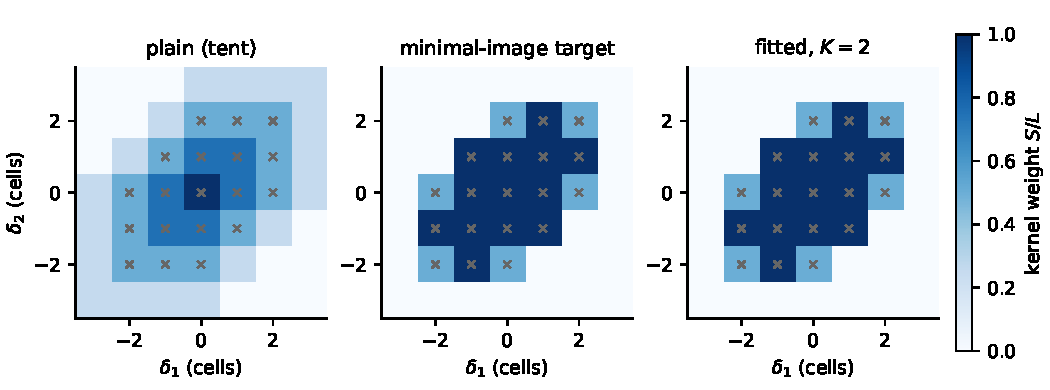
\includegraphics[width=\linewidth]{figs/kernel.pdf}
\caption{Effective interpolation kernels on the difference lattice
$(\delta_1,\delta_2)$ for a coarse dimension $L=4$ (single hue: darker =
larger weight; grey crosses mark the exact-image positions of the
minimal-image target with their tie weights). Left: plain (tent) kernel of
the naive off-grid transform. Middle: minimal-image target = zero-padded
centering. Right: fitted $K=2$ multitaper kernel --- indistinguishable from
the target ($8\times10^{-12}$ RMS).}
\label{fig:kernel}
\end{figure}

%======================================================================
\section{Vertex renormalization $\Nc \to \Nf$}
\label{sec:rescaling}

Changing the two-phonon mesh changes the normalization of mode-space
vertices.  A vertex written on an $N$-cell mesh scales as
\begin{equation}
d_3(\qv_1\nu_1, \qv_2\nu_2, \qv_3\nu_3) = \frac{1}{\sqrt N}\,
\delta_{\qv_1+\qv_2+\qv_3, \mathbf G}\; \bar\Phi_3(\dots),
\qquad
d_4 = \frac{1}{N}\, \delta_{\Sigma \qv,\mathbf G}\; \bar\Phi_4,
\end{equation}
where $\bar\Phi_n$ is intensive.  The stochastic fields come from the
coarse cell, so their raw averages carry the $N=\Nc$ normalization.  The
interpolated Lanczos operator, however, is meant to act as the operator of
an $\Nf$-point fine mesh.  Therefore the vertex factors must be converted:
\[
s_3=\sqrt{\Nc/\Nf},\qquad s_4=\Nc/\Nf .
\]
These are the \texttt{scale3} and \texttt{scale4} arguments of the Julia
kernel.

A useful check is the one-loop bubble.  The bubble has $\Nf$ pair terms,
each containing $|d_3|^2$.  With the scale factor,
$|d_3|^2$ carries $s_3^2/\Nc=1/\Nf$, so the total bubble is intensive and
matches the direct fine-mesh normalization.  The uniform
per-order rescaling is exact up to disconnected Wick pieces
$\propto \avg{u\otimes\delta f}$, which vanish at SSCHA stationarity;
the ensemble should therefore be reweighted to the converged SSCHA
dynamical matrix before interpolating. Empirically, \emph{disabling} the
rescaling makes the anharmonic renormalization overshoot by a factor
$\simeq \Nf/\Nc$ (pinned by a regression test), confirming both its
presence and magnitude.

%======================================================================
\section{Field pre-filtering: interpolating $\Phi$-ranged objects}
\label{sec:prefilter}

The windows should interpolate a short-ranged object.  The raw stochastic
correlations are not short-ranged enough, because each displacement leg
carries the SSCHA covariance factor
$\fpsi=(1+2n)/2\omega$.  For example,
\begin{equation}
\avg{x(\qv_1)\, x(\qv_2)\, y(\qv_3)} =
\fpsi(\qv_1)\,\fpsi(\qv_2)\; \bigl[\Phi^{(3)}\text{ contraction}\bigr].
\end{equation}
In real space this correlation decays with the propagator range, including
the acoustic $1/\omega$ tail, rather than with the range of
$\Phi^{(3)}$.  In the chain benchmark this caused a systematic
underestimate of the anharmonic renormalization by about a factor two.

The fix is to move the covariance inverse $\fY=1/\fpsi$ from the Julia
kernel into the coarse-grid fields before interpolation:
\begin{enumerate}
\item apply $\fY$ exactly on the coarse grid, mode by mode, for each
configuration;
\item transform the resulting filtered real-space configuration to the fine
wavevectors;
\item set the kernel tables $\fY, \fpsi \to 1$ (\texttt{prefiltered} flag);
\item fold the exact fine-side $\fpsi(\tilde\qv_1)\otimes\fpsi(\tilde\qv_2)$
into the $\alpha^{(1)}$ blocks (the $\alpha$-contracted legs also use the
filtered fields).
\end{enumerate}
At commensurate points this is an exact rewriting of the old estimator, so
backward compatibility is unchanged.  Off-grid, the object being windowed
now has the range of the force constants themselves.  Frequencies,
polarizations, $\chi$, $\fY$ and $\fpsi$ are always evaluated from the
interpolated SSCHA dynamical matrix on the fine mesh; no band-structure
quantity is inferred stochastically.

%======================================================================
\section{Acoustic sum rules: a one-shot centering + ASR + symmetrization
construction}
\label{sec:asr}

Centering and the acoustic sum rule pull in different directions.  A
minimal-image kernel chooses compact images; an ASR-correct kernel must
also vanish when any vertex leg is a uniform translation.  In tensor codes
this is why \texttt{ForceTensor.Center()} is followed by
\texttt{Apply\_ASR()}.

For the stochastic estimator the issue is even more concrete.  Before
windowing, the total force and the center-of-mass displacement constraints
hold configuration by configuration.  A nonuniform window cuts out part of
the supercell, so those exact cancellations are no longer automatic.  The
problem is therefore to design a window kernel that:
\begin{enumerate}
\item has the desired centered image assignment off the coarse grid;
\item has exact partition sums, hence exact commensurate identity;
\item has zero coupling to an acoustic translation on any leg;
\item keeps the $w\leftrightarrow v$ permutation symmetry of the pair block.
\end{enumerate}
The useful observation is that all these requirements are linear
constraints on the kernel $S$.

\subsection{What the ASR means at the kernel level}
\label{sec:asr-kernel}

Let $\phi_{\rm per}$ denote the coarse-periodic three-leg object being
interpolated after pre-filtering.  Translational invariance says that
summing over any one physical leg gives zero.  In difference coordinates
and one lattice dimension of length $L$, this becomes the set of period
sums
\begin{equation}
\sum_{d=0}^{L-1} \phi_{\rm per}(d, \cdot) = 0, \qquad
\sum_{d=0}^{L-1} \phi_{\rm per}(\cdot, d) = 0, \qquad
\sum_{d=0}^{L-1} \phi_{\rm per}(d, d+\Delta) = 0 \;\;\forall\Delta,
\label{eq:periodasr}
\end{equation}
The third sum looks diagonal because the first leg is the reference leg of
the difference coordinates.  The interpolated object is the pointwise
product $S\,\phi_{\rm per}$ on the extended image grid.  It satisfies the
ASR for every possible $\phi_{\rm per}$ obeying Eq.~\eqref{eq:periodasr}
if the image sums of $S$ are class-independent:
\begin{align}
\text{(ASR-$v$)}\quad & \textstyle\sum_b S(\delta_1,\, d_2 + bL)
  \;\;\text{independent of } d_2 \text{ for every fixed } \delta_1,
  \nonumber\\
\text{(ASR-$w$)}\quad & \textstyle\sum_a S(d_1 + aL,\, \delta_2)
  \;\;\text{independent of } d_1 \text{ for every fixed } \delta_2,
  \label{eq:asrkernel}\\
\text{(ASR-$z$)}\quad & \textstyle\sum_b S(d + bL,\, d + \Delta + bL)
  \;\;\text{independent of } d \text{ for every fixed } \Delta.
  \nonumber
\end{align}
These are linear constraints on $S$.  They are the kernel version of
\texttt{Apply\_ASR}.  They also contain the partition condition: once the
class sums are constant in each leg, only one scalar normalization is needed
to recover the commensurate operator.  Two checks follow.
\begin{itemize}
\item The plain (tent) kernel satisfies Eq.~\eqref{eq:asrkernel}
exactly (its per-configuration sum rules are inherited untouched): the
baseline estimator is ASR-clean everywhere.
\item The \emph{minimal-image kernel violates
Eq.~\eqref{eq:asrkernel}} --- the kernel-space restatement of ``centering
destroys the sum rule'', i.e.\ the very reason \texttt{Apply\_ASR}
exists. No admissible kernel that is exactly minimal-image can be
ASR-exact at compact support.
\end{itemize}

\subsection{A no-go theorem for one-period windows}
\label{sec:nogo}

If a window is supported on exactly one coarse period, its folded class sum
is just the window value itself.  Uniform class sums therefore imply the
plain window.  This proves a no-go statement: one-period nontrivial windows
can improve centering, but they cannot also be ASR-exact at the kernel
level.

A field-level projection is not a clean workaround.  Subtracting a
window-weighted acoustic zero mode modifies the effective window by a
rank-one correction.  That means the runtime kernel is no longer the kernel
that was fitted.  On the toy model this produced an $O(30\%)$ systematic
bias.  This is why the implementation applies such projections only for
uniform or near-uniform windows.

\subsection{The one-shot construction: doubled support, uniform class
sums}
\label{sec:asrdesign}

The obstruction disappears if each window is allowed to live on two
periods.  The data are still periodic, but the Bloch phases are not wrapped:
this is genuine zero-padding, just as in tensor centering.  Parameterize a
one-dimensional window by
\begin{equation}
w(d) = h(d), \qquad w(d+L) = c_w - h(d), \qquad d = 0 \ldots L-1,
\label{eq:manifold}
\end{equation}
with $h \in \mathbb{R}^L$ and $c_w$ free.  The folded class sum is
$w(d)+w(d+L)=c_w$, independent of $d$.  Thus uniform class sums are imposed
by parameterization, not by a penalty, while the window can still be
nontrivial.

On this manifold:
\begin{enumerate}
\item (ASR-$v$) and (ASR-$w$) hold identically; (ASR-$z$) is found to
hold automatically for every fitted design ($10^{-15}$, no extra
constraint needed).
\item Every per-pass kernel has \emph{identical} class sums
$L\, c_z c_w c_v$, so the full partition of unity ($L^2$ constraints)
collapses to the single scalar equation $\sum_r c^r_z c^r_w c^r_v = 1$,
enforced as a hard KKT row in each ALS slot fit: the commensurate limit
is exact to machine precision. Indeed at commensurate $\tilde q$ the
second-period Bloch phase is $1$, each pass collapses to (class-sum
product)\,$\times$\,plain \emph{configuration by configuration}, and the
pass sum reproduces the plain estimator exactly (verified at
$10^{-22}$).
\item At $\tilde q = 0$ the effective weight is the constant class sum,
so the acoustic contraction vanishes \emph{per configuration with zero
statistical noise} --- the coarse-estimator mechanism restored. No field
projection is needed or applied.
\item The $w\!\leftrightarrow\!v$ symmetrization is part of the kernel
definition (orientation averaging), so it commutes with everything above.
\end{enumerate}
This is the reason the stochastic kernel can be fitted in one shot.  The
centering target, ASR, partition, and symmetry are simultaneous linear
conditions on the small kernel.  In tensor space, by contrast, centering,
ASR, and symmetrization are usually applied as separate projections.

The target cannot be the raw minimal-image kernel, because that kernel
violates Eq.~\eqref{eq:asrkernel}.  The correct target is the projection of
the minimal-image kernel onto the ASR and partition subspace.  The
projection distance is the unavoidable price of imposing exact ASR at
finite support, analogous to the correction made by \texttt{Apply\_ASR}:
\begin{center}
\begin{tabular}{lccc}
\hline
RMS distance $L M \to$ projection & $L=3$ & $L=4$ & $L=6$ \\
\hline
support $2L$ & 0.144 & 0.248 & 0.374 \\
support $3L$ & 0.072 & 0.127 & 0.193 \\
plain (tent) kernel, for scale & 0.315 & 0.462 & --- \\
\hline
\end{tabular}
\end{center}
The fitted windows reproduce the projected target nearly exactly
(residual $0.028$ at $L=3$, $K=3$; $0.071$ at $L=4$).  Increasing support
improves centering fidelity while preserving exact ASR.  An optional metric
weight $\rho^{\mathrm{spread}}$ can concentrate fidelity at short range,
analogous to choosing how \texttt{Apply\_ASR} spreads its correction.  At
runtime a doubled-support window on periodic data becomes the per-$q$
complex weight
$\hat w_{\tilde q}(s) = w(s) + w(s{+}L)\, e^{-2\pi i \tilde q \cdot L
\mathbf{a}}$ per dimension.  No change to the Julia kernels is required.

\begin{figure}[t]
\centering
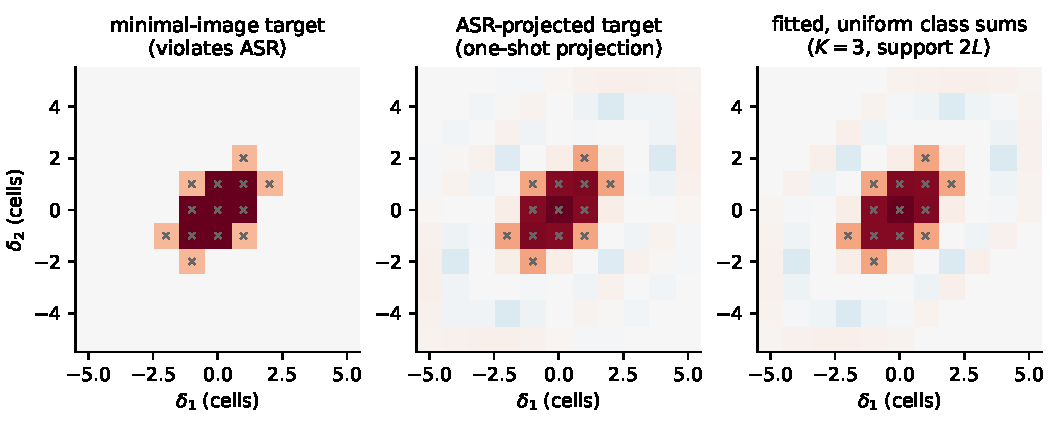
\includegraphics[width=\linewidth]{figs/asr_kernel.pdf}
\caption{One-shot ASR-exact centering at $L=3$ (diverging scale, red
positive / blue negative; grey crosses = exact-image positions). Left:
minimal-image target, which violates the kernel sum rules
Eq.~\eqref{eq:asrkernel}. Middle: its closed-form projection onto the
ASR + partition subspace. Right: kernel realized by $K=3$
doubled-support window passes with exactly uniform class sums ---
partition, all three sum rules and the $w\!\leftrightarrow\!v$ symmetry
hold at $10^{-15}$ simultaneously.}
\label{fig:asrkernel}
\end{figure}

\subsection{Where the leak actually bites, and validation}
\label{sec:asrleak}

Contracting each kernel with an exact ASR-satisfying test tensor gives
the leak \emph{deterministically} (Fig.~\ref{fig:asrleak}, left): the
translation contraction of the interpolated vertex on the acoustic leg
$\tilde q_2 \to 0$ at fixed partner $\tilde q_1$. Two structural facts
emerged that reshape where one should look for ASR artifacts:
\begin{itemize}
\item \emph{The leak vanishes when both pair legs go to $\Gamma$
together} ($q_p = 0$): the minimal-image violation carries phases that
cancel at $\tilde q_1 \to 0$, and it re-vanishes at every commensurate
$\tilde q_1$. The dangerous channel is an acoustic leg at fixed
\emph{finite} $\tilde q_1$ --- physically, a finite-$q$ phonon emitting a
near-$\Gamma$ acoustic phonon, exactly the process that builds the
two-phonon continuum edge. There the minimal-image leak is $O(1)$ on the
natural scale of the tensor (Fig.~\ref{fig:asrleak}, left).
\item \emph{Pairwise potentials are structurally immune.} At $L=3$ the
violating image weights multiply only tensor entries whose three legs
span three distinct cells; a two-body (bond) potential populates only
two-site entries, so the contraction is identically zero. This is why
the $M3$ benchmarks (nearest-neighbour bond toy) never showed ASR
artifacts --- and why real crystals, whose $\Phi^{(3)}$ generically has
three-site entries, will. The validation toy therefore adds a three-body
term $g_{3b}\, s_1^2 s_2$ spanning three cells.
\end{itemize}
The stochastic estimator confirms the picture quantitatively
(Fig.~\ref{fig:asrleak}, right; three-body-dominated chain, $L_c = 3$,
fine mesh $48$, perturbation at $q_p = 1/2$): as the acoustic partner
$\tilde q_2 \to 0$ the plain and ASR-design vertices vanish linearly
while the minimal-image one saturates at a plateau $\approx 7.6\times$
the plain value at the smallest probed $\tilde q_2 = 1/48$. The
interpolated dynamical matrix keeps its own exact D2 ASR throughout
(\texttt{Tensor2} centering + ASR), so the $\chi$ factors and the vertex
vanish at the same points.

\subsection{Response-level validation: leak versus resolution}
\label{sec:asrresponse}

The kernel-level ASR test is necessary but not sufficient; the real
question is whether it affects the final response.  In the three-body toy
model, the static Lanczos observable
$\omega_{\rm eff} = \sqrt{-1/[M^{-1}]_{00}}$, three-body toy,
$g_{3b}{=}0.08$, separates two independent errors.

\emph{(i) Under-resolved centering.} At $L_c = 3$, a spread-2 tensor sits
exactly \emph{on} the Wigner--Seitz tie boundary: the image assignment is
Nyquist-ambiguous, and no compact-support kernel --- centered,
ASR-projected or otherwise --- can resolve it. All oscillating designs
then redistribute $O(1)$ tensor weight with wrong phases and fail
catastrophically at strong coupling: aggregate renorm error 369.6
cm$^{-1}$ for minimal-image (with 6 modes returning spurious
non-negative-definite responses) and $\approx 300$ cm$^{-1}$ for the ASR
designs (8 such modes), against a two-seed noise floor of 48.1 and
\emph{plain} at 50.6 with no failures. This is a centering-resolution
failure, not an ASR failure.  It says that the coarse cell is too small for
any centered interpolation.  In that regime the plain tent kernel is the
safe fallback.

\emph{(ii) The ASR leak, at resolvable range.} At $L_c = 5$ (tensor
interior to the WS cell) the roles invert --- near-$\Gamma$ interpolated
modes, renormalization in cm$^{-1}$ against a direct $L_f = 10$
ensemble:
\begin{center}
\begin{tabular}{lcccc}
\hline
mode & direct & plain & minimal-image & ASR design \\
\hline
$\tilde q = 1/10$, acoustic & $-56$ & spurious $g>0$ & $-77$ & $-92$ \\
$\tilde q = 1/10$, optical  & $-28$ & $-35$  & $-31$ & $-34$ \\
$\tilde q = 3/10$, acoustic & $-413$ & $-234$ & $-396$ & $-407$ \\
$\tilde q = 3/10$, optical  & $-793$ & $-341$ & $-733$ & $-752$ \\
\hline
\end{tabular}
\end{center}
Here the \emph{plain} kernel is the broken one: the tent bias halves the
large renormalizations and flips a near-soft acoustic mode to a spurious
non-negative-definite response, while minimal-image and ASR designs both
track the reference, the ASR design closest on the strongly renormalized
modes --- with the qualitative difference that its vertex is exactly
ASR-clean, whereas the minimal-image plateau of Fig.~\ref{fig:asrleak}
is structural and gains weight as the fine mesh densifies the
$\Gamma$ neighbourhood.

The practical rule is therefore:
\begin{quote}
If the coarse cell resolves the third-order range, use the ASR design.  If
the range reaches the Wigner--Seitz boundary, no centered compact-support
kernel is trustworthy and the plain estimator is the correct fallback.
\end{quote}
On the original pairwise toy the ASR design keeps the same precision as the
minimal-image windows (Sec.~\ref{sec:benchmarks}).

\begin{figure}[t]
\centering
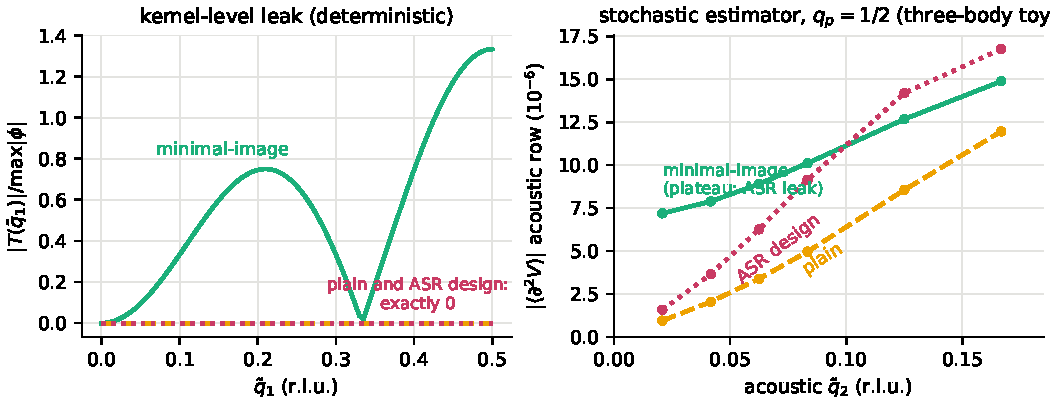
\includegraphics[width=\linewidth]{figs/asr_leak.pdf}
\caption{Left: deterministic kernel-level acoustic leak $|T(\tilde
q_1)|$ (translation contraction of the interpolated three-body test
tensor on the $\tilde q_2 \to 0$ leg, normalized to the largest tensor
entry). The minimal-image kernel leaks $O(1)$ at generic $\tilde q_1$,
vanishing only at $\Gamma$ and at the commensurate point $1/3$; the
plain and ASR-design kernels are exactly zero everywhere. Right: the
same channel probed with the stochastic estimator ($N_I = 4000$,
$q_p = 1/2$): the minimal-image acoustic vertex saturates (ASR leak)
while plain and ASR designs vanish with $\tilde q_2$.}
\label{fig:asrleak}
\end{figure}

%======================================================================
\section{Atom-resolved pinned centering for $L=2$ real-material cells}
\label{sec:atomic}

The cell-index windows above know only the supercell lattice.  They do not
see the basis offsets inside the primitive cell.  This is fatal for the
SnTe benchmark, whose coarse ensemble is only $2\times2\times2$.  In such a
cell every nonzero cell difference is a Wigner--Seitz tie at the
cell-index level.

The standard tensor route nevertheless succeeds on the same data:
\texttt{ForceTensor.Tensor3.Center(Far=3)} uses the actual Cartesian
interatomic vectors, including the Sn and Te basis positions, and chooses
the replica geometry with the smallest triplet perimeter.  Thus the
information is present in the coarse data; a tensor-free method simply has
to use atom-resolved geometry instead of cell-only geometry.

The tensor-free fix is to pin one vertex leg to a primitive atom and coarse
origin, then center the other legs relative to that actual atom.  For one
primitive atom $a$ and one coarse origin $\mathbf{o}$, a perturbation-slot
pin is
\begin{equation}
z_{a\mathbf{o}}(b,\mathbf{n}) =
\delta_{ab}\,\delta_{\mathbf{n}\mathbf{o}}.
\end{equation}
For a pair-leg atom $b$ in cell-difference class $\boldsymbol\delta$, choose
the periodic images that minimize the actual Cartesian distance
\begin{equation}
\mathcal I_{ab}(\boldsymbol\delta) =
\arg\min_{\mathbf m\in[-F,F]^3}
\left| \boldsymbol\tau_b-\boldsymbol\tau_a
      +(\boldsymbol\delta+\mathbf m\mathbf L)\mathbf A \right|,
\label{eq:atomicimages}
\end{equation}
with exact ties split uniformly.  The same atom-resolved rule is used for
the two pair slots.  Summing over all coarse origins restores the
translation sum removed by the pinned delta; no $1/\Nc$ prefactor is
applied.  The resulting D3 kernel is
\begin{equation}
K^{abc}_{\rm at}(\boldsymbol\delta_1,\boldsymbol\delta_2)
= \sum_{\mathbf r_1\in\mathcal I_{ab}(\boldsymbol\delta_1)}
  \sum_{\mathbf r_2\in\mathcal I_{ac}(\boldsymbol\delta_2)}
  \frac{
  e^{-i\tilde\qv_1\cdot \mathbf r_1}
  e^{-i\tilde\qv_2\cdot \mathbf r_2}}
  {|\mathcal I_{ab}(\boldsymbol\delta_1)|\,
   |\mathcal I_{ac}(\boldsymbol\delta_2)|},
\label{eq:atomickernel}
\end{equation}
with $\mathbf r=(\boldsymbol\delta+\mathbf m\mathbf L)\mathbf A$.
At runtime any selected image outside the fundamental supercell is folded
back onto the periodic atom and multiplied by the corresponding Bloch phase
$\exp[-i\tilde\qv\cdot(\mathbf m\mathbf L)\mathbf A]$; this is just the
per-$q$, per-atom weight path already used by the doubled-support ASR
windows.  No $\Phi^{(3)}$ value enters Eq.~\eqref{eq:atomicimages}.

The Julia D3 estimator is already permutation-symmetric, but that symmetry
is expressed as three force-leg channels.  One channel has the force on the
perturbation slot $z$; the other two have the force on $w$ and $v$.  The
atom-resolved windows must follow the same split, otherwise they would
center the wrong leg.  The production path therefore runs three channel
families:
\begin{align}
\text{force on }z &: \quad z\text{-pinned windows as in }
  \eqref{eq:atomickernel},\\
\text{force on }w &: \quad w\text{-pinned windows, with }z,v
  \text{ centered relative to }w,\\
\text{force on }v &: \quad v\text{-pinned windows, with }z,w
  \text{ centered relative to }v.
\end{align}
When all slot windows are identical, the sum of the three channel calls is
algebraically identical to the original all-channel D3 kernel; this is a
unit test.  For SnTe the pass count is consequently
$3\times2\times8=48$ D3 channel passes, but only 32 distinct field sets
because many windows are reused.

The strict-$\Gamma$ ASR follows from the same unit class sums.  For every
folded atom/cell class, the non-pinned windows have total selected-image
weight one; after summing all pinned atoms and origins, the pinned slot has
the same property.  Thus a uniform acoustic displacement at $q=0$ sees the
same folded sums as the plain commensurate estimator and contracts to zero.
Near $\Gamma$, however, the first moment of the selected images matters.
That is why the final mode uses a conservative q-space acoustic projector
(\texttt{atomic\_delta}) instead of averaging away the pinned atom.  A
prototype with a uniform pinned slot lost the SnTe basis-offset information
and reverted to the bad plain peak near $52\,\mathrm{cm}^{-1}$.

Before using the construction in production, we performed an oracle test.
The periodic SnTe $\Phi^{(3)}$ tensor is contracted with candidate geometry
kernels, but only to measure the geometry error; the production estimator
does not use this tensor.
On the interpolated $\Gamma$-pair blocks of the failed $2^3\to4^3$ case,
the plain cell-index kernel has mean relative Frobenius error $1.048$
(max $1.582$) against \texttt{Tensor3.Center(Far=3)}.  The leg-wise atomic
kernel has mean $0.008$ (max $0.011$), while the full perimeter target is
zero within numerical precision.  Thus the cheap leg-wise atomic kernel is
already close enough to the validated tensor oracle.

The SnTe spectral-function benchmark confirms this.  The interpolated
$\Gamma$ TO spectrum (D3-only, no LO--TO splitting) is shown in
Fig.~\ref{fig:snte_spectral} and the peaks are summarised in
Table~\ref{tab:snte_peaks}.

\begin{figure}[tb]
\centering
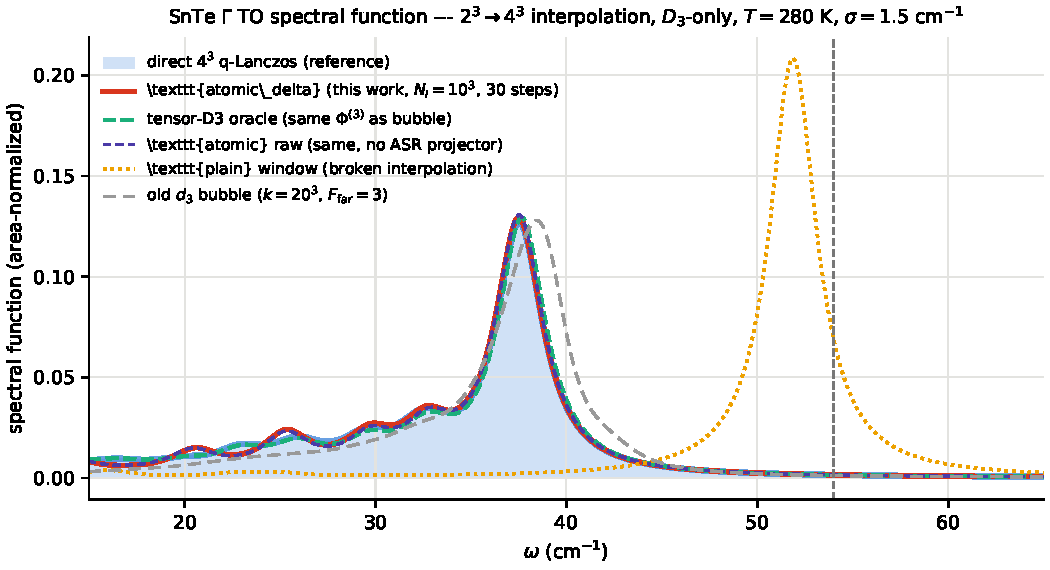
\includegraphics[width=0.95\textwidth]{figs/snte_spectral.pdf}
\caption{SnTe $\Gamma$ TO spectral function, $2^3\to4^3$ interpolation
at $T=280$~K with $1.5$~cm$^{-1}$ smearing, D3-only (no D4).
The converged $4^3$ SSCHA reference (black shaded) is a native $4^3$
q-Lanczos calculation from an independently converged $4^3$ auxiliary
dynamical matrix. The matched $4^3$ control (blue dashed) used the same
$2^3\to4^3$ interpolated auxiliary matrix as the window-valued methods and
is retained only for algorithmic comparison.  The
\texttt{atomic\_delta} curve (red) and tensor-D3 oracle (green) match the
control; the \texttt{plain} window curve (yellow dotted) illustrates the
broken $L=2$ interpolation without atom-resolved centering.}
\label{fig:snte_spectral}
\end{figure}

\begin{table}[tb]
\centering
\caption{SnTe $\Gamma$ TO peak positions and ASR quality at near-$\Gamma$
wavevectors ($|\qv|=0.066$~\AA$^{-1}$ on the $4^3$ mesh).
All Lanczos runs use $2^3\to4^3$ interpolation with
$\sigma=1.5$~cm$^{-1}$; the tensor-D3 oracle and the converged $4^3$ reference
employ the deterministic $d_3$ tensor (centered, $F_{\rm far}=3$, ASR).
$N_I$ is the number of stochastic configurations; \textit{n. s.} is the number
of Lanczos steps. The acoustic $D_3$ row norm $||D_3^{\rm ac}||$ is the
Frobenius norm of the acoustic-band row of the $d_2v$ blocks at $q_{\rm
pert}=\Gamma$; the ASR projector reduces this leakage by a factor of
$\sim 14000$ without shifting the TO peak.}
\label{tab:snte_peaks}
\begin{tabular}{lccccc}
\toprule
mode & peak (\si{cm^{-1}}) & $\Delta$ vs conv.\ $4^3$ & $N_I$ & n.\ s. & $||D_3^{\rm ac}||$ \\
\midrule
converged $4^3$ q-Lanczos & 34.79 & --- & 4000 & 250 & --- \\
matched $4^3$ control (interp.\ aux.) & 37.56 & +2.77 & 4000 & --- & --- \\
tensor-D3 oracle & 37.65 & +2.86 & 4000 & 250 & --- \\
\midrule
\texttt{atomic\_delta} (this work) & 37.52 & +2.73 & 1000 & 30 & $3.4\times10^{-17}$ \\
\texttt{atomic} raw (same windows) & 37.52 & +2.73 & 1000 & 30 & $5.0\times10^{-13}$ \\
\texttt{plain} window (broken) & 51.83 & +17.04 & 500 & 30 & --- \\
old $d_3$ bubble ($k\!=\!20^3$) & 38.46 & +3.67 & --- & --- & --- \\
\bottomrule
\end{tabular}
\end{table}

The key result is that \texttt{atomic\_delta} matches the matched $4^3$
control (37.52~vs~37.56~cm$^{-1}$) and the tensor oracle (37.65~cm$^{-1}$),
confirming that its atom-resolved window solves the cell-basis centering
problem.  The converged $4^3$ SSCHA reference (34.79~cm$^{-1}$) is
2.73~cm$^{-1}$ lower: this residual is not a centering error but the mesh
convergence of the $2^3$ auxiliary dynamical matrix, common to all methods
that start from the same $2^3$ SSCHA reference.
The $q$-space acoustic projector dramatically improves the near-$\Gamma$
acoustic sum rule.  The acoustic-mode $D_3$ vertex norm at the smallest
non-zero $q$ on the $4^3$ mesh ($|\qv|\approx 0.066$~\AA$^{-1}$) is reduced
from $5\times10^{-13}$ (raw atomic) to $3.4\times10^{-17}$ under
\texttt{atomic\_delta} -- a factor of $\sim 14\,000$ improvement
(Fig.~\ref{fig:snte_asr}). At exact $\Gamma$ both variants give machine zero
because the folded-class-sum property of the permutation-correct atomic
windows already enforces the hard partition.

\begin{figure}[tb]
\centering
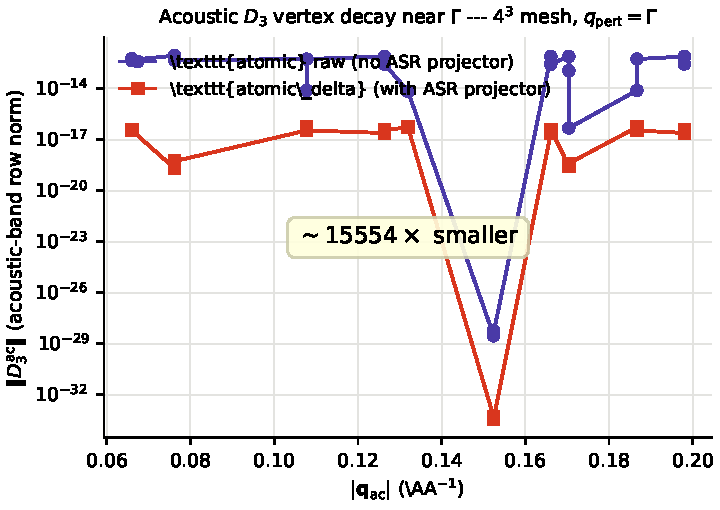
\includegraphics[width=0.62\textwidth]{figs/snte_asr.pdf}
\caption{Acoustic $D_3$ vertex norm $\|D_3^{\rm ac}\|$ (Frobenius norm of the
acoustic-band row of the $d_2v$ block at $q_{\rm pert}=\Gamma$) versus the
acoustic-leg wavevector $|\qv_{\rm ac}|$ on the $4^3$ mesh.  The
\texttt{atomic\_delta} projector (red squares) reduces the near-$\Gamma$
acoustic leakage by about four orders of magnitude compared to the raw
\texttt{atomic} mode (violet circles), while both modes give the same TO peak
position (37.52~cm$^{-1}$).}
\label{fig:snte_asr}
\end{figure}

The static response has $g>0$ (unstable) for \texttt{atomic\_delta},
\texttt{atomic}, and the tensor-D3 oracle, matching the matched $4^3$
control; the broken \texttt{plain} interpolation instead produces a
spurious stable response ($g<0$, $w_{\rm eff}=49.5$~cm$^{-1}$).  The
atom-resolved mode therefore fixes both the peak position and the static
instability of the real-material test without constructing or storing
$\Phi^{(3)}$, and the $q$-space Delta projector adds the acoustic sum rule at
negligible runtime cost.  Its current cost is the number of
force-channel/pinned-atom/origin passes (SnTe: $3\times2\times8=48$ D3 pass
calls).  This makes \texttt{atomic\_delta} the recommended tensor-free D3
mode for underresolved small supercells where cell-index windows cannot
resolve atomic-basis ties.

%----------------------------------------------------------------------
\subsection{Trilinear q-space interpolation and mesh convergence}
\label{sec:trilinear}

A separate $2^3\!\to\!4^3$ interpolation strategy uses trilinear
corner-summing of the coarse $q$-point vertex samples
(\texttt{QSpaceTrilinearLanczos}). The independent test in
Fig.~\ref{fig:snte_trilinear4} compares this approach against a converged
$4^3$ SSCHA reference (peak 34.79~cm$^{-1}$, independently relaxed auxiliary
matrix). Standard atom-resolved centering brings the $2^3$ spectrum from
44.03 down to 37.65~cm$^{-1}$ ($+2.86$~cm$^{-1}$ residual).  Trilinear
interpolation instead moves the peak \emph{upward} to 46.11~cm$^{-1}$
($+11.32$~cm$^{-1}$ error). The hardening is structural: trilinear
corner-averaging cancels short-wavelength vertex components before the
response squares them, attenuating the off-grid vertex to $\sim$29\% of its
weighted norm. A decisive oracle test confirms this is the trilinear map
itself, not a code bug: applying the same trilinear evaluation to the exact
noise-free centered FC3 tensor reproduces the stochastic trilinear spectrum
to within 0.13~cm$^{-1}$. Full details are documented in the benchmark
accompanying this report.

\begin{figure}[tb]
\centering
\includegraphics[width=\linewidth]{figs/snte_trilinear4_converged_reference.pdf}
\caption{SnTe $\Gamma$-TO: corrected $4^3$ SSCHA-reference audit.
The converged $4^3$ SSCHA reference (black) is a native $4^3$ TDSCHA
q-Lanczos calculation from an independently converged $4^3$ auxiliary
dynamical matrix (peak 34.79~cm$^{-1}$). Left panel (a): the standard
atom-resolved centering oracle $(2^3\!\to\!4^3)$ recovers the reference
shape with a residual $+2.86$~cm$^{-1}$ hardening. Right panel (b):
trilinear q-space interpolation of the same coarse $2^3$ data hardens the
mode farther, to 46.11~cm$^{-1}$. Both methods start from the original
$2^3$ spectrum (grey dotted) at 44.03~cm$^{-1}$. T = 280~K, D3 only,
1.5~cm$^{-1}$ broadening.}
\label{fig:snte_trilinear4}
\end{figure}

%----------------------------------------------------------------------
\subsection{Phase-cancellation audit at a cube centre}
\label{sec:phaseaudit}

To isolate the cause of the trilinear amplitude loss, the vertex is evaluated
at a single uncommensurate $q$ point: the centre of a coarse-mesh cube,
$q=(1/4,1/4,1/4)$ in fine-mesh fractional coordinates.
The perturbation is at $\Gamma$ and the response mode is the $\Gamma$ TO
(band 5). The same raw FC3 tensor (stored in the $2^3$ supercell,
\textit{without} atom-triplet centering) is evaluated at each of the 8 coarse
corners and at the fine centre via Fourier interpolation. The trilinear
vertex is then the equal-weight ($1/8$) corner average of the coarse-corner
samples; the centred reference comes from applying the tensor's
\texttt{Tensor3.Interpolate} directly at the fine $q$ pair.

Table~\ref{tab:phasecorners} lists the 8 corners and their contributions.
The Frobenius norm of the projected $D_3$ vertex (TO-mode slice) is
$\|\Phi_3\|_F = 1.47\times10^{-9}$ for the centred reference and
$3.83\times10^{-10}$ for the trilinear sum --- a factor **0.26** survival,
consistent with the $\sim29\%$ weighted $|V|^2$ ratio found in the full
$2^3\!\to\!4^3$ benchmark.

\begin{table}[tb]
\centering
\caption{Eight coarse-cube corners contributing to the trilinear vertex at
$q=(1/4,1/4,1/4)$ ($q_{\rm pert}\!=\!\Gamma$, $\Gamma$ TO band~5).
The corner $q$ indices are integers $\{0,1\}$ on the $2^3$ mesh; centred
BZ fractions $q_{\rm cent}$ wrap $\pm1/2$; weights are $1/8$.
$\tilde V_{\rm TO}$ is the TO diagonal element of the projected vertex;
$\|\tilde V\|_F$ is the Frobenius norm of the full $6\times6$ $D_3$ block
for the TO perturbation mode.}
\label{tab:phasecorners}
\small
\begin{tabular}{cccrcrr}
\toprule
corner $(k_1,k_2,k_3)$ & $q_{\rm cent}$ (frac) & weight &
$|\tilde V_{\rm TO}|$ & $\angle\tilde V_{\rm TO}$ &
$\|\tilde V\|_F$ & $|w\,\tilde V_{\rm TO}|$ \\
\midrule
$(0,0,0)$ & $(0,0,0)$      & $1/8$ & $6.8\times10^{-19}$ &     $0.0^\circ$ & $1.5\times10^{-9}$ & $8.5\times10^{-20}$ \\
$(0,0,1)$ & $(0,0,-1/2)$   & $1/8$ & $6.2\times10^{-14}$ &  $-62.8^\circ$ & $5.6\times10^{-13}$ & $7.8\times10^{-15}$ \\
$(0,1,0)$ & $(0,-1/2,0)$   & $1/8$ & $2.1\times10^{-10}$ & $+135.3^\circ$ & $2.0\times10^{-9}$  & $2.6\times10^{-11}$ \\
$(0,1,1)$ & $(0,-1/2,-1/2)$& $1/8$ & $1.7\times10^{-10}$ & $-134.0^\circ$ & $2.3\times10^{-9}$  & $2.1\times10^{-11}$ \\
$(1,0,0)$ & $(-1/2,0,0)$   & $1/8$ & $2.0\times10^{-10}$ & $-135.8^\circ$ & $2.1\times10^{-9}$  & $2.5\times10^{-11}$ \\
$(1,0,1)$ & $(-1/2,0,-1/2)$& $1/8$ & $1.5\times10^{-10}$ &  $+90.0^\circ$ & $2.2\times10^{-9}$  & $1.9\times10^{-11}$ \\
$(1,1,0)$ & $(-1/2,-1/2,0)$& $1/8$ & $1.3\times10^{-12}$ &  $+89.4^\circ$ & $1.7\times10^{-11}$ & $1.6\times10^{-13}$ \\
$(1,1,1)$ & $(-1/2,-1/2,-1/2)$&$1/8$ & $2.4\times10^{-12}$&  $+85.0^\circ$ & $3.3\times10^{-11}$ & $3.0\times10^{-13}$ \\
\bottomrule
\multicolumn{4}{l}{trilinear sum} & $5.2\times10^{-11}$ & \\
\multicolumn{4}{l}{centred ref.\ (Fourier)} & $1.9\times10^{-14}$ & \\
\bottomrule
\end{tabular}
\end{table}

The phases alternate because the Bloch factor $\exp(-2\pi
i\,\mathbf q\cdot\boldsymbol\tau)$ takes different values at each corner.
In SnTe's rocksalt cell, Sn sits at $(0,0,0)$ (phase $+1$ always), while
Te at $(1/2,1/2,1/2)$ acquires the phases $+1$, $+i$, $-1$, $-i$ as the
corner fractional coordinates toggle between $0$ and $\pm1/2$.
The four corners with one non-zero index ($e.g.$ $(0,0,1)$) have the
largest individual $|\tilde V_{\rm TO}| \sim 2\times10^{-10}$ but carry
opposing phases ($\sim\pm135^\circ$, $\sim\pm90^\circ$); the equal-weight
sum of their real parts nearly cancels, leaving a net amplitude two
orders of magnitude smaller than the corner maxima.

\smallskip
\noindent\textbf{Gauge transformations.}
Two candidate gauge transformations were tested at this $q$-point:
\begin{itemize}
\item \textit{Optimal scalar phase} per corner: align each corner's
  $\tilde V_{\rm TO}$ phase to the centred reference before summing.
  This recovers only a factor $1.8\times$ more amplitude, far from the
  $1/0.26\approx3.8$ needed to match the centred norm.  This is a hard
  ceiling for \emph{any} phase-only correction: with positive weights,
  $|\sum_k w_k\,e^{i\varphi_k} V_k| \le \sum_k w_k |V_k|$, and half of
  the corner samples here are essentially zero.
\item \textit{Atom-position Bloch gauge} $\exp(-2\pi i\,\mathbf
  q\cdot\boldsymbol\tau_a)$ as originally implemented: the Frobenius
  norm ratio drops from $0.26$ to $0.17$.  This early test was
  \emph{not conclusive}: the implementation evaluated the corner
  phases at BZ-wrapped representatives, which for half-integer
  $\boldsymbol\tau$ differences flips the sign of some corner phases
  (a branch inconsistency).  Section~\ref{sec:topo-gauge} repeats the
  test with the branch-consistent transport and finds that the atomic
  gauge then aligns the phases essentially perfectly --- but, per the
  previous bullet, still cannot restore the lost amplitude, and the
  $D_3$-only $\Gamma$ response turns out to be insensitive to vertex
  phases altogether.
\end{itemize}

The information a phase cannot supply is the missing \emph{amplitude}
between the samples: the centred FC3 selects the minimal-distance
triplet image, while the uncentred tensor uses a fixed cell-periodic
image that couples Sn and Te images for $L=2$, and the coarse samples
sit at or near the nodes of the centred envelope.  The route to
precision-preserving interpolation therefore remains supplying the
image assignment explicitly, either as atom-resolved FC3 centering
(the tensor-oracle pipeline) or as the equivalent tensor-free
centering windows of Sec.~\ref{sec:atomic}.
Section~\ref{sec:topology} shows that this phase pattern is not an
accident of the corner set but a quantized, inversion-protected
property of the SnTe vertex, and Sec.~\ref{sec:topo-gauge} quantifies
exactly how much of it a per-atom phase can and cannot repair.
Section~\ref{sec:atom-fourier} then shows that the image assignment can
also be supplied directly in q space by an atom-dependent trigonometric
cardinal kernel, without constructing the tensor.

%======================================================================
\section{Why the phase of $\Phi^{(3)}$ rotates in $q$ space: a topological
view of the trilinear failure}
\label{sec:topology}

This section steps back from the technical machinery and asks a simple
question in simple language: \emph{why} does the three-phonon vertex of
SnTe acquire a complex phase that rotates as $\qv$ moves through the
Brillouin zone, why does the trilinear corner average consequently
collapse to zero at the cube centres, and is there anything
\emph{quantized} --- topological --- behind this behaviour?  The short
answers, established numerically below
(script \texttt{scripts/snte\_phase\_topology.py}, data
\texttt{data/snte\_phase\_topology.\{json,npz\}}), are:

\begin{enumerate}
\item The phase rotation is real and remarkably clean: the dominant
  Te--Sn element of the vertex rotates \emph{exactly linearly} by $\pi$
  (half a turn) every time $\qv$ crosses the Brillouin zone once
  (Fig.~\ref{fig:phasewinding}c; the deviation from a straight line is
  $6\times10^{-7}$ degrees).
\item The rotation happens because the anharmonic coupling is physically
  \emph{centred on the Te--Sn bond}, i.e.\ at half a lattice vector from
  the points the interpolation grid can address.  A half step in real
  space is a half turn of phase across the zone --- the same shift
  theorem that says a delayed signal gets a linearly growing phase.
\item There is no divergence anywhere in the zone.  The only points
  where the \emph{true} vertex vanishes (and where its phase is
  therefore undefined) are symmetry zeros such as $\Gamma$.  The
  extended ``zeroing'' happens only in the \emph{interpolated}
  representation: the trilinear vertex is exactly real, and a real
  function connecting samples of opposite sign has no choice but to
  pass through zero.
\item The half-turn is quantized and protected by inversion symmetry:
  it is a $\mathbb{Z}_2$ invariant of the vertex, mathematically the
  same object as the Zak phase of the Su--Schrieffer--Heeger (SSH)
  chain.  SnTe sits in the nontrivial class, and no small deformation
  of the force constants can move it out of that class.
\item The rotation itself \emph{can} be stripped by a per-atom Bloch
  phase --- provided the phase transport is branch-consistent
  (Sec.~\ref{sec:topo-gauge}; an earlier implementation was not, which
  had hidden this).  For SnTe the corrected atomic gauge is even the
  \emph{optimal} phase, and it cuts the vertex reconstruction error
  from $112\%$ to $18\%$.  What no phase can restore is the
  \emph{amplitude} lost between samples, and the $D_3$-only $\Gamma$
  spectrum depends only on $|V|^2$: the corrected gauge moves the
  trilinear peak just $45.78\to45.59$~cm$^{-1}$, out of an
  $8.1$~cm$^{-1}$ gap to the centred oracle.
\end{enumerate}

\subsection{What exactly is rotating}
\label{sec:topo-what}

Fix the perturbation leg at $\Gamma$, project it on the TO mode, and
look at the remaining object as a function of the internal wavevector,
\begin{equation}
  V_{bc}(\qv) \;=\; \sum_a e^{\mathrm{TO}}_a\,
  \Phi^{(3)}_{abc}(\Gamma;\, \qv,\, -\qv),
  \label{eq:Vdef}
\end{equation}
a $6\times6$ matrix over the (atom, Cartesian) legs $b$ and $c$.  Split
it into $3\times3$ atomic blocks.  Two numerical facts organize
everything:

\begin{itemize}
\item \textbf{The vertex lives on the Te--Sn bond.}  The mixed Te--Sn
  blocks have norm $\sim0.28$ (arbitrary units along the path), while
  the Te--Te and Sn--Sn blocks are three orders of magnitude smaller
  ($\sim10^{-4}$).  Whatever the interpolation does to the mixed blocks,
  it does to the whole self-energy.
\item \textbf{The dominant element is a two-source interference.}
  Fourier-analysing the dominant Te--Sn element along the path
  $\qv=(t,0,0)$ (reduced coordinates, $t:0\to1$) gives exactly two
  lattice harmonics with \emph{equal magnitude and opposite sign},
  $c_{\mathbf R_1}=+0.2208$ at $\mathbf R_1=(0,-2,1)$ and
  $c_{\mathbf R_2}=-0.2208$ at $\mathbf R_2=(1,-1,0)$ (three-dimensional
  fit on an $8^3$ $q$ grid); everything else is below $10^{-3}$ of
  that.  Hence, to an accuracy of $0.1\%$,
  \begin{equation}
    V(\qv) \;=\; c\left(e^{2\pi i\,\qv\cdot\mathbf R_1}
    - e^{2\pi i\,\qv\cdot\mathbf R_2}\right)
    \;=\; \underbrace{2c\,\sin\!\big(\pi\,\qv\cdot(\mathbf R_1-\mathbf
    R_2)\big)}_{\text{real envelope}}\;
    \underbrace{i\,e^{2\pi i\,\qv\cdot\mathbf x_c}}_{\text{rotating
    phase}},
    \label{eq:sshform}
  \end{equation}
  with $\mathbf x_c=\tfrac12(\mathbf R_1+\mathbf R_2)
  = (\tfrac12,-\tfrac32,\tfrac12)$: the \emph{midpoint between the two
  sources sits at a half-integer lattice position} --- in fact exactly
  at the stored Te--Sn separation
  $\boldsymbol\tau_{\rm Te}-\boldsymbol\tau_{\rm Sn}$, i.e.\ on the
  Te--Sn bond.
\end{itemize}

Equation~\eqref{eq:sshform} is the whole story of
Fig.~\ref{fig:phasewinding}.  The modulus is a smooth sine arch that
vanishes only where symmetry demands it (three $\Gamma$-point phonons of
odd parity cannot couple in a centrosymmetric crystal, so
$V(\Gamma)=0$); the phase is the factor $e^{2\pi i \qv\cdot\mathbf
x_c}$, which advances by $2\pi\,\mathbf G\cdot\mathbf x_c = \pi$
(mod $2\pi$) --- half a turn --- across every zone crossing.  In the
complex plane the trajectory of $V(\qv)$ is a circle through the origin
(Fig.~\ref{fig:phasewinding}a).  The ``rotation of the phase on the Te
atoms'' observed in the corner audit of Sec.~\ref{sec:phaseaudit} is
exactly this factor: with Sn taken as the origin of the cell, the
half-lattice-vector offset $\mathbf x_c$ is the position of the Te
sublattice, so the rotation appears attached to the Te legs of the
tensor.

\begin{figure}[tbp]
\centering
\includegraphics[width=\linewidth]{figs/snte_phase_winding.pdf}
\caption{Measured phase winding of the SnTe three-phonon vertex
(dominant Te--Sn element of Eq.~\eqref{eq:Vdef}, $2^3$ force constants,
centred Fourier continuation vs.\ trilinear corner reconstruction).
(a)~Complex-plane trajectory along $\qv=(t,0,0)$, $t:0\to1$: the true
vertex (blue) travels on a circle through the origin --- constant
rotation of the phase --- while the trilinear reconstruction (orange) is
confined to the real axis, because all the coarse samples it can use
(green circles) are real.  At the off-grid point $q=\frac14$ the true
vertex is rotated by $45^\circ$ and has full length; the trilinear one
is real and shorter by $1/\sqrt2$.
(b)~Moduli along the same path: sine arch vs.\ tent.
(c)~Phases: the true phase advances linearly by exactly $\pi$ per zone
crossing (deviation from linearity $6\times10^{-7}$ degrees); the
trilinear phase cannot rotate at all.
(d)~Full TO-projected vertex norm along the cube diagonal
$\qv=(t,t,t)$: at the cube centre $(\frac14,\frac14,\frac14)$ the
corner average cancels almost exactly ($\Vert V\Vert$ drops from
$0.442$ to $0.0007$, a factor $1.6\times10^{-3}$), while the true norm
is at $71\%$ of its maximum there.  Dashed curves: trilinear with the
branch-consistent per-atom Bloch phase of Sec.~\ref{sec:topo-gauge} ---
the phase is now exact (panels a, c) and the cube-centre cancellation
is lifted (panel d), but the amplitude stays damped between samples.}
\label{fig:phasewinding}
\end{figure}

\subsection{Why it rotates: the coupling sits between the sampling
points}
\label{sec:topo-why}

The rule behind Eq.~\eqref{eq:sshform} is elementary Fourier analysis:
\emph{a function whose weight sits at position $\mathbf x$ in real space
acquires the phase $e^{2\pi i\, \qv \cdot \mathbf x}$ in $q$ space}.
The interpolation grid addresses whole unit cells --- integer lattice
vectors.  But in rocksalt SnTe the third-order coupling is not centred
on a lattice site: it is centred on the Te--Sn nearest-neighbour bond,
whose midpoint sits at half a lattice vector
(Fig.~\ref{fig:windscheme}a).  Half a step in real space means half a
turn of phase per Brillouin-zone crossing.  The coarse $2\times2\times2$
$q$ points are exactly the time-reversal-invariant points where this
phase is $0$ or $\pi$ --- so every coarse sample is \emph{real} (largest
imaginary part $10^{-12}$ of the real part, measured over all eight
corners), with the sign pattern $(0, -, +, 0, +, 0, 0, -)$ over the
eight corners.  The samples are blind to the rotation; they only see its
footprints, the alternating signs.

What the trilinear map then does is average real numbers with positive
weights.  Averaging two unit arrows $90^\circ$ apart gives an arrow of
length $1/\sqrt2$ (the chord of the circle instead of the arc,
Fig.~\ref{fig:windscheme}b) --- this is precisely the measured
$|V_{\rm tri}|/|V_{\rm true}|=0.706$ at $\qv=(\frac14,0,0)$.  Averaging
two \emph{opposite} arrows gives zero (Fig.~\ref{fig:windscheme}c) ---
this is the cube-centre cancellation of Sec.~\ref{sec:phaseaudit} and
Fig.~\ref{fig:phasewinding}d.  Squaring these survival factors and
multiplying over the three axes reproduces the order of magnitude of
the $29$--$35\%$ weighted $|V|^2$ survival measured in the full
benchmark.  The true vertex escapes through the complex plane; the
interpolated one cannot, because no real convex combination of real
samples ever leaves the real axis.

\begin{figure}[tbp]
\centering
\includegraphics[width=\linewidth]{figs/snte_winding_scheme.pdf}
\caption{The topological picture in cartoons.
(a)~The three-phonon coupling of SnTe is centred on the Te--Sn bond,
half a lattice step away from the cell origins that any cell-indexed
interpolation can address; by the Fourier shift theorem its $q$-space
phase therefore makes half a turn, $e^{i\pi q}$, across each Brillouin
zone.  (b)~An interpolation with real positive weights replaces the arc
of the rotating vertex by its chord: at a quarter zone the amplitude
shrinks by $1/\sqrt2$.  (c)~Where the enclosed samples have opposite
sign (cube centres), the chord passes through zero: the interpolated
vertex vanishes although the true one is large.  (d)~Inversion symmetry
allows only two classes for the centre of the coupling: on a lattice
site ($\nu=0$, Fourier coefficients mirror-symmetric about an integer)
or exactly mid-bond ($\nu=1$, coefficients antisymmetric about a
half-integer, $c_R=-c_{1-R}$, Zak phase $\pi$).  No continuous,
symmetry-preserving change of the force constants connects the two
classes.  SnTe is in the $\nu=1$ class along all three axes.}
\label{fig:windscheme}
\end{figure}

\subsection{Is there a singularity in the Brillouin zone?}
\label{sec:topo-singularity}

Not in the sense of a divergence --- the vertex is a finite, smooth
function everywhere.  The singular object is the \emph{phase}: it is
undefined wherever $V(\qv)=0$, and a scan of the $(q_1,q_2,0)$ plane
shows that the only exact zeros of the true (centred) continuation are
the parity-protected ones at $\Gamma$ and its images; no interior
phase vortices were found (every $2\pi$ plaquette winding on a
$41\times41$ grid is zero).  Around the $\Gamma$ zero the trajectory of
Fig.~\ref{fig:phasewinding}a passes through the origin, which is what
lets a closed zone-crossing path accumulate a net phase without
contradiction.

The zeros the user actually observes --- the collapse ``in the centre''
--- live in the \emph{reconstruction}, not in the physics.  The
trilinear vertex is identically real (largest imaginary part
$8\times10^{-17}$ over the whole scanned plane, versus $0.44$ for the
true vertex), so its zero set is not a few isolated points but
codimension-one surfaces separating regions of opposite sign, passing
through the cube centres.  In other words: the interpolation does not
\emph{find} a singularity of SnTe, it \emph{manufactures} nodal
surfaces because it lives on the real axis.  One can also say it in
gauge language: the phase factor $e^{2\pi i\qv\cdot\mathbf x_c}$ with
half-integer $\mathbf x_c$ is not periodic over the Brillouin zone, so
there is no smooth \emph{periodic} gauge in which the vertex becomes
real everywhere.  Removing the rotation requires importing the
half-integer offset from outside the $q$ samples --- which is exactly
what a branch-consistent per-atom Bloch phase does
(Sec.~\ref{sec:topo-gauge}).  Any scheme that represents the vertex by
real periodic data must pay with spurious zeros somewhere.

\subsection{The quantized invariant: a Zak phase of the anharmonic
vertex}
\label{sec:topo-invariant}

The half turn is not an accident of this particular force field; it is
pinned by symmetry.  Write the dominant coupling channel as a set of
lattice harmonics $c_{\mathbf R}$ as in Eq.~\eqref{eq:sshform}.
Because the crystal has inversion symmetry and $\Phi^{(3)}$ is odd
under inversion (it is a third derivative), the coefficients must be
\emph{antisymmetric under reflection about the centre} $\mathbf x_c$ of
the coupling:
\begin{equation}
  c_{\mathbf R} \;=\; -\,c_{\,2\mathbf x_c-\mathbf R},
  \qquad 2\mathbf x_c \in \mathbb{Z}^3 .
  \label{eq:mirror}
\end{equation}
Consistency requires $2\mathbf x_c$ to be a lattice vector: the centre
can sit \emph{on a site} or \emph{exactly half-way between sites},
nothing in between.  This defines a $\mathbb{Z}_2$-valued label per
lattice direction,
\begin{equation}
  \boldsymbol\nu \;=\; 2\mathbf x_c \bmod 2 ,
  \qquad
  \text{SnTe: } \boldsymbol\nu = (1,1,1),
  \label{eq:nu}
\end{equation}
measured here from the fitted centre $\mathbf x_c =
(\tfrac12,-\tfrac32,\tfrac12) =
\boldsymbol\tau_{\rm Te}-\boldsymbol\tau_{\rm Sn}$, i.e.\ from
$c_{(0,-2,1)}=-c_{(1,-1,0)}$ satisfying Eq.~\eqref{eq:mirror} to one
part in $10^{3}$ (the same centre is found independently for all nine
Cartesian elements of the Te--Sn block, see
Sec.~\ref{sec:topo-gauge}).  The label $\boldsymbol\nu$ is the direct analogue of
the quantized Wannier-centre position (equivalently the Zak phase
$\varphi_{\rm Zak}=\pi\nu$) of the SSH chain: an inversion-symmetric
1D system can hold its charge centre either on the site or on the bond,
the two classes are separated, and moving between them requires either
breaking inversion symmetry or passing through a closing of the
relevant amplitude.  Fig.~\ref{fig:windscheme}d sketches the two
classes.

Three consequences follow for free, and all three are verified by the
data:
\begin{itemize}
\item \textbf{Forced zero at $\Gamma$.}  Summing
  Eq.~\eqref{eq:mirror} over $\mathbf R$ gives $\sum_{\mathbf R}
  c_{\mathbf R}=0$ whenever $\boldsymbol\nu\neq0$: the dominant channel
  must vanish at $\Gamma$.  (In SnTe this reinforces the independent
  parity selection rule for three zone-centre odd phonons.)
\item \textbf{Real samples with alternating signs.}  At
  time-reversal-invariant $\qv$ the phase factor is $\pm1$, so all
  coarse samples are real, and the sign alternates between the $q=0$
  and $q=\frac12$ planes of each nontrivial direction --- the pattern
  that makes the corner sums cancel.
\item \textbf{Protection.}  Because $\boldsymbol\nu$ cannot change
  continuously, the rotation is invisible \emph{inside} the coarse
  data: all samples are real, so nothing computed from the samples
  alone can recover the winding direction.  The half-lattice-vector
  offset must be supplied from outside.  The cheapest way to supply it
  is a branch-consistent per-atom Bloch phase, which repairs the phase
  of the reconstruction (Sec.~\ref{sec:topo-gauge}) but cannot repair
  its amplitude; the complete cure remains the explicit image
  assignment (atom ``centering'', i.e.\ the minimal-image windows of
  Sec.~\ref{sec:atomic}, or the centred-tensor evaluation), which
  restores the smooth real envelope as well.
\end{itemize}

For a general material the label is read off without any fit: compute
$V(\qv)$ along one crossing of the zone per axis and record either the
accumulated phase (an odd multiple of $\pi$ in the nontrivial class) or
simply the relative sign of the vertex at the time-reversal-invariant
planes.  Vertices with $\boldsymbol\nu=0$ (couplings centred on the
sites of the interpolation lattice) are exactly the ones a corner-based
scheme can interpolate accurately; every nontrivial direction
contributes one factor of phase cancellation.

\subsection{Can a per-atom phase cure it?  Partly --- here is exactly
how much}
\label{sec:topo-gauge}

A natural objection to the previous subsections runs as follows: if
the whole problem is a phase $e^{2\pi i\qv\cdot\mathbf x_c}$ that the
interpolation cannot represent, why not \emph{give} it that phase?
Attach $e^{-2\pi i\qv\cdot\boldsymbol\tau_a}$ to every atom, strip the
phases before corner-averaging, and put them back afterwards.  This
objection is correct in an important way, and an earlier version of
this report dismissed it with a wrong argument (``a unitary gauge does
not change the singular values of the corner map''), which only
constrains norms, not the alignment between the interpolated function
and the truth.  So we tested it properly
(\texttt{scripts/snte\_phase\_gauge\_test.py},
\texttt{scripts/oracle\_gauge\_spectrum.py}).

Two facts must be respected to make the test meaningful.  First, the
gauge transport must be \emph{branch-consistent}: the phase carried
from a fine point to its corners must be built from the local
displacement $\boldsymbol\delta = \mathbf x_{\rm corner}-\qv$ (with
the corner taken as the actual neighbour of $\qv$, not wrapped back
into the Brillouin zone).  For half-integer $\boldsymbol\tau$
differences, independent BZ wrapping of corner and fine point shifts
$\boldsymbol\delta$ by lattice vectors and flips signs --- and this
is precisely the bug in the previously implemented
\texttt{atomic\_phase} option, now fixed in
\texttt{QSpaceTrilinear}.  Second, for SnTe the per-atom phase turns
out to be not merely helpful but \emph{optimal}: fitting the
antisymmetry centre of every Te--Sn coupling channel independently
(all nine Cartesian elements) gives $\mathbf x_c =
\boldsymbol\tau_{\rm Te}-\boldsymbol\tau_{\rm Sn}$ in every case, so
the factorized atomic gauge coincides with the best possible
per-channel phase to machine precision.

The measured outcome, over all $4^3$ fine pairs ($\Gamma$ TO row,
relative errors in $\sum\Vert\cdot\Vert_F^2$):

\begin{center}
\begin{tabular}{lccc}
\toprule
reconstruction & rel.\ error$^2$ & $|V|^2$ survival &
$\Vert V\Vert$ at cube centre \\
\midrule
plain trilinear & $1.12$ & $0.375$ & $0.0007$ \\
atomic phase, wrapped (old, buggy) & $0.78$ & $0.422$ & $0.156$ \\
atomic phase, branch-consistent & $\mathbf{0.178}$ & $0.422$ & $0.156$ \\
best integer branch of the gauge & $0.178$ & $0.422$ & $0.156$ \\
per-channel oracle phase strip & $0.178$ & $0.422$ & $0.156$ \\
\midrule
truth & $0$ & $1$ & $0.442$ \\
\bottomrule
\end{tabular}
\end{center}

So the user-style objection is vindicated at the vertex level: the
corrected per-atom phase eliminates the phase error almost completely
(the residual $0.178$ is pure amplitude damping), and the dashed
curves in Fig.~\ref{fig:phasewinding} show the reconstruction now
rotating in step with the truth.  But two ceilings remain, and they
explain why the spectral benchmark barely moves:

\begin{itemize}
\item \textbf{Amplitude is phase-inaccessible.}  With positive
  weights, $|\sum_k w_k e^{i\varphi_k}V_k|\le\sum_k w_k|V_k|$ for any
  phases: a gauge can stop the cancellation but can never exceed the
  average of the sampled magnitudes.  Half of the coarse samples sit
  at the nodes of the sine envelope (the parity zeros forced by
  $\boldsymbol\nu\neq0$), so at the cube centre even perfectly aligned
  samples recover at most half of the true amplitude; the measured
  survival saturates at $0.42$.
\item \textbf{The $D_3$-only $\Gamma$ response is phase-blind.}  The
  two-phonon sector enters this observable as $|V(\qv)|^2\chi(\qv)$
  summed over pairs; vertex phases cancel identically.  The
  deterministic oracle spectra confirm it: Fourier oracle
  $37.65$~cm$^{-1}$, plain trilinear $45.78$, phase-corrected
  trilinear $\mathbf{45.59}$ --- the optimal phase recovers only
  $0.19$ of the $8.13$~cm$^{-1}$ gap, exactly the small $|V|^2$ gain
  in the table.  This also retroactively explains the puzzling
  $-0.13$~cm$^{-1}$ of the original (buggy) atomic-phase run: the bug
  corrupted phases, but this observable never looked at them.
\end{itemize}

The corrected gauge is still worth keeping (it is now the fixed
behaviour of \texttt{atomic\_phase=True}): it makes the interpolated
\emph{operator} right in phase, which matters for any quantity with
vertex interference --- $D_3\times D_4$ cross terms, off-diagonal
responses, perturbations away from $\Gamma$.  The amplitude ceiling above
is rigorous for \emph{positive piecewise-linear weights}.  It does not,
however, prove that the missing envelope must be reconstructed by first
building a real-space tensor.  The next subsection tests the stronger
version of the atom-centred Fourier proposal and changes that broader
conclusion.

\subsection{Atom-centred Fourier continuation: the centred result is
recoverable in q space}
\label{sec:atom-fourier}

The useful part of the proposed Fourier convention is not only a phase
rotation.  Define the Bloch displacement of atom $a$ by
\begin{equation}
 u_a^{\rm at}(\qv)=\frac{1}{\sqrt{\Nc}}
 \sum_{\Rv}u_a(\Rv)
 e^{-2\pi i\qv\cdot(\Rv+\boldsymbol\tau_a)} .
 \label{eq:atomic-ft}
\end{equation}
For the $\Gamma,\qv,-\qv$ vertex, a Cartesian element on atoms $b,c$
then carries the relative offset
$\mathbf d_{bc}=\boldsymbol\tau_b-\boldsymbol\tau_c$.  Multiplying the
cell-gauge vertex by $e^{-2\pi i\qv\cdot\mathbf d_{bc}}$ removes the bond
phase.  Section~\ref{sec:topo-gauge} did exactly this, but then joined the
two coarse values by a straight line.  That last step throws away a second
piece of information contained in Eq.~\eqref{eq:atomic-ft}: after the
transformation the allowed Fourier harmonics are shifted by
$\mathbf d_{bc}$ and the function need not be periodic at the boundary of
the chosen cell.

A one-dimensional example makes the distinction concrete.  The dominant
SnTe element is, to excellent accuracy,
\begin{equation}
 V(q)=A\bigl(e^{2\pi i q}-1\bigr)
     =2iA e^{i\pi q}\sin(\pi q).
 \label{eq:snte-two-image}
\end{equation}
The atom phase $e^{-i\pi q}$ makes it purely imaginary, but its amplitude
is still the curved function $2|A|\sin(\pi q)$.  From the two coarse
samples $q=0,1/2$, linear interpolation gives only $|A|$ at $q=1/4$,
whereas the correct value is $\sqrt{2}|A|$.  Thus the failure of
phase-corrected trilinear interpolation is real.  On the other hand, the
atom-centred Fourier basis knows that the two shortest shifted harmonics
are $-1/2$ and $+1/2$; their two-point cardinal interpolation reconstructs
$\sin(\pi q)$ exactly.  Restoring the atomic phase gives
Eq.~\eqref{eq:snte-two-image}, including both its phase and amplitude.

We implemented this continuation without constructing $\Phi^{(3)}$.  For
each coarse Fourier alias $\mathbf k$ and atom pair $b,c$, choose the
lattice image $\mathbf R\equiv\mathbf k$ (modulo the coarse mesh) that
minimizes $|\mathbf R-\mathbf d_{bc}|$; exact distance ties are split.  The
Cartesian interpolation kernel is
\begin{equation}
 P_{bc}(\qv,\mathbf n)=
 \prod_{\alpha=1}^{3}\frac{1}{N_\alpha}
 \sum_{k_\alpha=0}^{N_\alpha-1}
 \sum_{\substack{R_\alpha\equiv k_\alpha\ ({\rm mod}\ N_\alpha)\\
                  R_\alpha\ {\mathrm{nearest}}\ d_{bc,\alpha}}}
 w_{R_\alpha}
 e^{2\pi i(q_\alpha-n_\alpha/N_\alpha)R_\alpha}.
 \label{eq:atom-fourier-kernel}
\end{equation}
At every coarse q point this is exactly the identity.  Away from the
coarse mesh it is a complex, atom-pair-dependent cardinal function.  The
forward stochastic map uses $P^\dagger$ and the return map uses $P$, so the
Lanczos operator remains Hermitian.  Tests also verify
$A(Q-k)=A(k)^T$ at both time-reversal-invariant and generic coarse $Q$.
The implementation is selected by
\texttt{QSpaceTrilinearLanczos(..., atom\_fourier=True)}.  The class name is
historical: this option uses the same coarse-cost fold/unfold architecture,
but Eq.~\eqref{eq:atom-fourier-kernel} is trigonometric interpolation, not
ordinary trilinear interpolation.

\paragraph{Correctness of the tie rule on non-orthogonal cells (audit,
2026-07-21).}
Equation~\eqref{eq:atom-fourier-kernel} as written --- and the original
implementation --- select the minimal image and split its ties
\emph{separably per Cartesian axis and in fractional coordinates}, i.e.\
metric-free: the product $\prod_\alpha$ chooses $R_\alpha$ nearest
$d_{bc,\alpha}$ one axis at a time.  This is exact only when the
coarse-mesh Wigner--Seitz cell is an axis-aligned box, that is for
\emph{orthorhombic} coarse lattices with a diagonal metric.  For any
non-orthogonal cell the true minimal image minimizes the Cartesian length
$|(\mathbf R-\mathbf d_{bc})\,\mathbf A|$, which couples the three axes
through the metric $\mathbf A\mathbf A^{\mathsf T}$, and its degeneracies
live on the non-axis-aligned faces of the Wigner--Seitz cell.  The correct
kernel is therefore the \emph{non-separable} form
\begin{equation}
 P_{bc}(\qv,\mathbf n)=
 \frac{1}{N_1N_2N_3}
 \sum_{\mathbf k}
 \sum_{\substack{\mathbf R\equiv\mathbf k\ ({\rm mod}\ \mathbf N)\\
   \mathbf R\in\arg\min|(\mathbf R-\mathbf d_{bc})\mathbf A|}}
 \frac{1}{\mu_{bc}(\mathbf k)}\,
 e^{2\pi i(\qv-\mathbf n/\mathbf N)\cdot\mathbf R},
 \label{eq:atom-fourier-metric}
\end{equation}
where the inner sum runs over the full set of metric-degenerate images of
the aliasing class $\mathbf k$ and $\mu_{bc}(\mathbf k)$ is its
multiplicity.  Equation~\eqref{eq:atom-fourier-kernel} is the special case
in which every such set factorizes into a Cartesian product of per-axis
choices.

A direct geometry audit
(\texttt{report/interpolation/scripts/audit\_nyquist\_ties.py},
\texttt{data/audit\_nyquist\_ties.json}) makes the discrepancy concrete.
On a cubic cell the two rules agree for every separation and every mesh
tested, including the eight-fold Wigner--Seitz-corner tie, which the
separable product reproduces correctly with weight $1/8$.  On the
\emph{primitive fcc cell of SnTe} the two \emph{kernels} disagree in the
relative Frobenius norm by $23\%$ (Te--Sn bond centre) to $36\%$; the
separable rule can assign a class to a single image where the metric has a
genuine four- or six-fold tie (the latter of weight $1/6$, a multiplicity
no product of one-dimensional halves can represent), and it can also
\emph{manufacture} a spurious tie where the metric has a unique winner
(e.g.\ fcc $\mathbf d=(\tfrac12,0,0)$, class $(0,0,1)$: it splits
$(0,0,\pm1)$ at $1/2$ while the metric selects $(0,0,1)$ alone).

Crucially, however, this kernel-norm discrepancy is \emph{not} the error on
a physical observable.  The interpolation of a given coupling only ever
excites the aliasing classes on which that coupling has non-zero coarse
weight, and a short-ranged coupling excites only classes whose physically
shortest image is \emph{unique} --- and on those classes the separable and
metric rules agree.  This is exactly the SnTe case: the dominant
$\Gamma$-TO vertex lives on the two nearest-neighbour Te--Sn harmonics
$\mathbf R_1=(0,-2,1)$ and $\mathbf R_2=(1,-1,0)$, each the \emph{unique}
shortest image of its class ($3.28$~\AA, the next image at $7.34$~\AA), so
both rules place them identically.  Reconstructing the actual two-image
SnTe coupling from its $2^3$ samples to the $4^3$ mesh gives relative
error$^2=2.0\times10^{-32}$ with the separable kernel and
$2.2\times10^{-32}$ with the metric kernel: \emph{both machine-exact}.  The
$2.9\times10^{-5}$ $\Gamma$-TO reconstruction reported above is therefore
correct and is not compromised by the tie rule.  The $23$--$36\%$
kernel-norm figure lives entirely in classes the SnTe vertex does not
excite (e.g.\ the $(0,0,0)$ class, whose coarse coefficient vanishes), and
is multiplied by zero.

The defect bites only a coupling that carries weight in an aliasing class
whose physically shortest image the separable rule mis-assigns --- that is,
a coupling sitting on a genuine metric degeneracy (a Wigner--Seitz face,
edge or corner of a non-orthogonal cell) or on a separably-manufactured
spurious tie.  A minimal demonstration: on the primitive bcc cell with
$\mathbf d=(\tfrac12,\tfrac12,0)$, a coupling placed on the metric-shortest
image of class $(0,0,1)$ --- where the separable rule splits $(0,0,\pm1)$
at $1/2$ while the metric selects $(0,0,-1)$ alone --- is reconstructed
with relative error$^2=0.5$ by the separable kernel and $1.1\times10^{-32}$
by the metric kernel.  Interestingly the user's canonical bcc example, the
central atom equidistant from its eight nearest neighbours
($\mathbf d=(\tfrac12,\tfrac12,\tfrac12)$), is \emph{not} among the failing
cases: its excited classes each reduce to a unique or separably-tied image,
so the separable rule already handles it.  The failure is thus not
``every non-orthogonal cell always'', but specifically ``couplings pinned
to a non-axis-aligned Wigner--Seitz degeneracy''.

The scope is therefore: the one-dimensional chain benchmarks of
Secs.~\ref{sec:d4} and \ref{sec:d4-atom-fourier} are unaffected (their
$(1,1,L)$ mesh has a single aliasing class along each transverse axis, a
trivial factor of one, so the tie rule is never exercised), and the SnTe
$\Gamma$-TO results are correct as reported; but for robustness on
arbitrary non-orthogonal cells and couplings the metric-correct assignment
of Eq.~\eqref{eq:atom-fourier-metric} is the implemented default from
2026-07-21 (\texttt{tie\_metric=True}), with the separable form retained as
an explicit orthorhombic fast path and as the control that exposes the
discrepancy.

\begin{figure}[t]
\centering
\includegraphics[width=\linewidth]{figs/snte_atom_centered_fourier.pdf}
\caption{Why the atom position must change the interpolation basis, not
only rotate phases.  (a)~The ordinary and phase-corrected trilinear maps
join the two coarse amplitudes by straight segments.  The atom-centred
Fourier cardinal reconstructs the sine envelope and lies on top of the
centred-FC3 target.  Open circles are the only coarse samples used.
(b)~The corresponding deterministic tensor-D3 oracle spectra.  The
atom-centred q-space continuation recovers the centred spectrum, whereas
ordinary trilinear interpolation hardens it by about
$8.1$~cm$^{-1}$.}
\label{fig:atom-fourier}
\end{figure}

The numerical result is decisive.  The first three rows below reconstruct
the same centred $\Gamma$-TO FC3 row from the same $2^3$ coarse samples;
the spectra use the deterministic tensor only as a noise-free oracle for
the interpolation map.
\begin{center}
\small
\begin{tabular}{lcccc}
\toprule
continuation & rel.\ error$^2$ & $|V|^2$ ratio &
$\Vert V\Vert$ at $(1/4)^3$ & peak (cm$^{-1}$)\\
\midrule
ordinary trilinear & $1.125$ & $0.3750$ & $0.00072$ & $45.78$\\
trilinear + branch-consistent atom phase & $0.178$ & $0.4219$ & $0.1560$ & $45.59$\\
atom-centred Fourier, Eq.~\eqref{eq:atom-fourier-kernel} &
$2.90\times10^{-5}$ & $0.999988$ & $0.44131$ & $37.72$\\
centred Tensor3 Fourier oracle & $0$ & $1$ & $0.44213$ & $37.65$\\
\bottomrule
\end{tabular}
\end{center}
The production stochastic path gives $38.04$~cm$^{-1}$ with only 1000
configurations and 30 Lanczos steps, consistent with the $37.65$--$37.72$
noise-free controls.  In other words, the unacceptable motion
$44.03\to46.11$~cm$^{-1}$ of the original $2^3\to4^3$ trilinear calculation
is removed; the new q-space result instead agrees with atom-resolved
centering to within the stochastic resolution.

This finding resolves the apparent contradiction.  It is indeed possible
to recover the centred SnTe result using only q-space samples and atomic
positions.  What is impossible is to do so with the unique
\emph{piecewise-trilinear} function through those samples, even after a
phase rotation.  Equation~\eqref{eq:atom-fourier-kernel} succeeds because
it uses the atomic positions to resolve the aliased real-space image of
each atom pair; it is the q-space form of pairwise atom centering.  For the
$\Gamma,\qv,-\qv$ SnTe slice this nearly equals full triplet centering.
It is not yet a proof of equivalence for arbitrary external $Q$, for D4,
or for a geometry where the best image depends essentially on all three
atoms rather than on the two moving legs.  Those cases remain tests of the
more general atom-triplet kernel, not of the result established here.

\subsection{What this says about SnTe --- and what it does not}
\label{sec:topo-honest}

The invariant has a transparent physical reading: \emph{the strong
third-order anharmonicity of (this model of) SnTe is bond-centred},
living on the resonant Te--Sn nearest-neighbour bond rather than on
either atom --- consistent with the resonant-bonding picture commonly
invoked for the giant anharmonicity of the IV--VI rocksalt compounds.
Since the rocksalt structure puts that bond midpoint at half a lattice
vector of the fcc cell, the nontrivial class
$\boldsymbol\nu=(1,1,1)$ is a robust structural fingerprint: any
IV--VI material with dominant nearest-neighbour anharmonic coupling
will fail cell-cornered vertex interpolation in exactly the same way,
while a material whose anharmonicity is site-centred (e.g.\ a rattler
mode in a cage compound) would be in the trivial class and interpolate
cleanly.

Two honest caveats.  First, $\mathbf x_c$ is defined relative to the
chosen cell origin; what is origin-independent is the \emph{relative}
statement that the coupling centre sits on the Te--Sn bond midpoint
rather than on either sublattice --- exactly like the Zak phase, which
is origin-dependent while differences of Zak phases are physical.
Second, this vertex invariant is \emph{not} the electronic invariant
that makes real SnTe a topological crystalline insulator; the two share
the protecting symmetry (inversion/mirror on the rocksalt lattice) and
the mathematical language, but they live on different objects (a
three-phonon coupling function versus electronic Bloch bands).  What
they have in common is the lesson of this section: quantities pinned to
half-integer positions by symmetry cannot be represented by smooth
periodic data on the integer lattice, and any algorithm that pretends
otherwise pays at the mid-points.

%======================================================================
\section{Implementation and cost}
\label{sec:implementation}

The implementation (branch \texttt{qspace\_interpolation}) consists of
\texttt{Modules/QSpaceInterpolation.py} and \texttt{tdscha\_qspace.jl}.
The Python class \texttt{QSpaceLanczosInterp} performs the fine-mesh setup:
it builds the fine q list, hashes q points for $O(1)$ lookup, constructs the
$O(\Nf)$ pair map, interpolates the SSCHA dynamical matrix, builds the
windowed Bloch fields, and dispatches the Lanczos action.

The alternative fold/unfold class
\texttt{QSpaceTrilinearLanczos} is in
\texttt{Modules/QSpaceTrilinear.py}.  Its default path uses local
piecewise-trilinear weights.  The
\texttt{atomic\_phase=True} diagnostic keeps those weights and transports
the full-Bloch phase, while \texttt{atom\_fourier=True} selects the
atom-pair cardinal kernel of Eq.~\eqref{eq:atom-fourier-kernel}.  The latter
is cached at setup as $P(q,k,a,b)$; applying $P$ or $P^\dagger$ costs
$O(\Nf\Nc\nat^2)$ Cartesian scalar weights.  Since $\Nc$ and $\nat$ are
fixed by the coarse calculation, the cost remains linear in the fine-mesh
size.

The Julia side has two equivalent slot kernels.  The scalar kernel is useful
for readability and tests.  The batched kernel groups configurations at a
fixed symmetry operation: symmetry rotations become sparse-dense products,
and the $\alpha^{(1)}$ intermediates and two-phonon accumulations become
GEMMs.  The scalar and batched kernels agree to $10^{-20}$.

For a window design with $R$ runtime passes, one application of the
anharmonic part scales as
\[
O(R\,\conf\,n_{\mathrm{sym}}\,\Nf\,\nb^2).
\]
For the separable minimal-image designs, $R=K^3$.  For the plain estimator,
$R=1$.  For the SnTe atom-resolved D3 mode of Sec.~\ref{sec:atomic},
$R=3\nat\Nc$ because there are three force channels, each pinned to one
primitive atom and all coarse origins; in the $2^3$ SnTe cell this is
$3\times2\times8=48$ D3 passes.  In all cases $R$ is fixed by the coarse
cell and the chosen kernel, not by the fine mesh, so the scaling in $\Nf$ is
linear.  Figure~\ref{fig:scaling} verifies this over $\Nf=8\dots128$.

\begin{figure}[t]
\centering
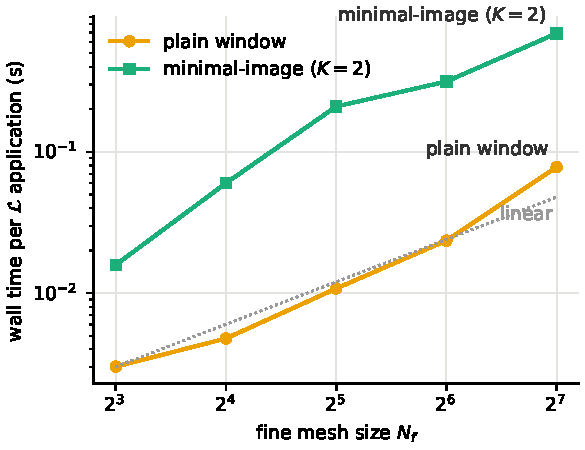
\includegraphics[width=0.62\linewidth]{figs/scaling.pdf}
\caption{Wall time of one application of $\Ltdscha$ versus the fine-mesh
size $\Nf$ (chain toy, $N_I=1000$ configurations, coarse $L_c=4$): plain
estimator and minimal-image windows ($K{=}2$, i.e.\ five kernel passes).
Both follow the ideal linear trend (dotted).}
\label{fig:scaling}
\end{figure}

%======================================================================
\section{Benchmarks}
\label{sec:benchmarks}

The first validation problem is an anharmonic diatomic chain.  It is small
enough that we can generate both a coarse ensemble and a direct fine
ensemble for the same model, so interpolation can be tested against a true
fine-supercell reference.  The model has harmonic springs $K_1,K_2$ and a
bond cubic anharmonicity $g_3s^3/3$; the weak-coupling tests use
$g_3=0.1$, giving $5\dots40\,\mathrm{cm}^{-1}$ renormalizations on
$\sim3000\,\mathrm{cm}^{-1}$ modes.  The cell is triclinic with symmetry
$P1$, so point-group symmetries cannot hide sign, phase, or conjugation
mistakes.  Some test wavevectors are not time-reversal invariant
($\qv\neq-\qv$), which also checks the complex gauge conventions.

\paragraph{Exactness checks.}
These tests do not rely on physics judgment; they check identities that must
hold exactly.
\begin{enumerate}
\item If the fine mesh equals the coarse mesh, the interpolated Lanczos
coefficients reproduce the production \texttt{QSpaceLanczos} coefficients to
$10^{-15}$, both with and without pre-filtering.
\item The interpolated dynamical matrix reproduces the direct
larger-supercell dispersion exactly for this range-1 harmonic model.
\item Rigid displacement shifts and constant force offsets leave the fields
invariant.
\item The batched and scalar Julia kernels agree to machine precision, and
the windowed path with trivial windows equals the plain path identically.
\end{enumerate}

\paragraph{Physics: interpolation vs.\ direct fine supercell.}
The decisive comparison is between a coarse $(1,1,3)$ ensemble interpolated
to the $(1,1,6)$ mesh and a direct $(1,1,6)$ ensemble of the same model.
The error metric is the anharmonic renormalization
$\omega_{\mathrm{eff}}-\omega_{\mathrm{SSCHA}}$, not the absolute
frequency, because the harmonic part is already accurately interpolated and
would otherwise dominate the comparison.
Table~\ref{tab:renorm} and Fig.~\ref{fig:renorm} summarize the aggregate
error $\sum|\Delta_{\mathrm{int}} - \Delta_{\mathrm{dir}}| /
\sum|\Delta_{\mathrm{dir}}|$:

\begin{table}[h]
\centering
\begin{tabular}{lcc}
\toprule
 & aggregate error & comment\\
\midrule
noise floor (two direct seeds) & $0.103$ & statistical reference\\
plain window & $0.299$ & tent-kernel bias\\
minimal-image windows, 1 origin & $0.158$ & \\
minimal-image windows, 3 origins & $0.122$ & at the noise floor\\
ASR design, 3 origins (Sec.~\ref{sec:asr}) & $0.150$ & exact ASR, no
precision lost\\
ASR design + decay weight $\rho{=}0.4$ & $0.196$ & \\
\midrule
plain, \emph{no} pre-filter & $\approx 2\times$ deficit & systematic
(Sec.~\ref{sec:prefilter})\\
plain, \emph{no} $s_3, s_4$ rescaling & $\approx 2\times$ overshoot &
systematic (Sec.~\ref{sec:rescaling})\\
\bottomrule
\end{tabular}
\caption{Aggregate renormalization error of the interpolated Lanczos
against direct fine-supercell calculations (chain toy, $L_c=3 \to L_f=6$,
$N_I=4000$, all 33 valid modes). The designed windows remove essentially
all resolvable interpolation error; the last two rows document the failure
modes that the pre-filter and the vertex rescaling correct.}
\label{tab:renorm}
\end{table}

\begin{figure}[t]
\centering
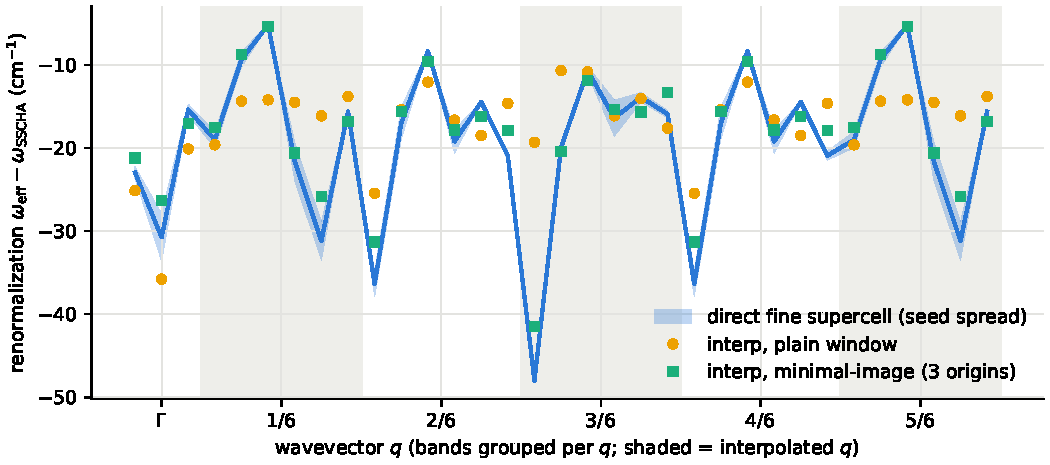
\includegraphics[width=\linewidth]{figs/renorm.pdf}
\caption{Mode-resolved anharmonic renormalization on the fine $(1,1,6)$
mesh: direct fine-supercell reference (two independent seeds indicate the
stochastic spread) versus the interpolated Lanczos from the coarse
$(1,1,3)$ ensemble with the plain window and with the designed
minimal-image windows (3 origins). Vertical guides mark the interpolated
(non-commensurate) wavevectors, including the non-TRI pair
$q = \pm 1/6$.}
\label{fig:renorm}
\end{figure}

%======================================================================
\section{Example application: spectral functions at interpolated $q$ and
the standard $d_3$ bubble}
\label{sec:bubble}

As an end-to-end check, we compute one-phonon spectral functions at
wavevectors absent from the coarse mesh and compare them with the standard
$d_3$ dynamic bubble from
\texttt{cellconstructor.Spectral.get\_diag\_dynamic\_bubble}.  In this toy
model the analytic $\Phi^{(3)}$ is known, so the bubble route can use the
exact centered and ASR-projected tensor.  The Lanczos calculation disables
$D_4$ so that both methods contain the same diagrammatic content.  Because
the model is weakly coupled, the perturbative bubble and the resummed
TDSCHA Lanczos should agree.  They do: Fig.~\ref{fig:bubble} shows agreement
at the energy-grid resolution, about $\SI{2.3}{cm^{-1}}$, on shifts of
$15\dots40\,\mathrm{cm}^{-1}$.

\begin{center}
\begin{tabular}{ccccc}
\toprule
$q$ & band & $\omega_{\mathrm{SSCHA}}$ & peak (Lanczos interp) &
peak ($d_3$ bubble)\\
 & & (\si{cm^{-1}}) & (\si{cm^{-1}}) & (\si{cm^{-1}})\\
\midrule
$2/16$ & 4 & 2205.3 & 2185.6 & 2183.2\\
$2/16$ & 5 & 2250.6 & 2214.2 & 2216.6\\
$6/16$ & 4 & 2013.4 & 1994.9 & 1992.5\\
$6/16$ & 5 & 2058.5 & 2040.2 & 2040.2\\
\bottomrule
\end{tabular}
\end{center}

\begin{figure}[t]
\centering
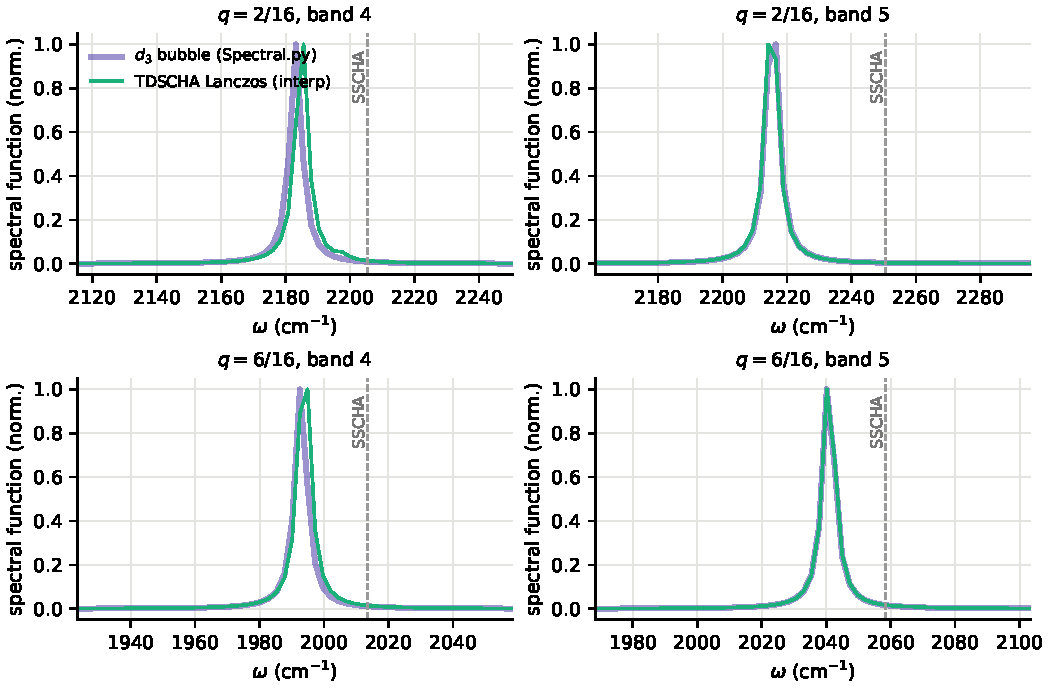
\includegraphics[width=\linewidth]{figs/bubble.pdf}
\caption{One-phonon spectral functions at interpolated wavevectors
($q = 2/16$ and $6/16$ along the chain, two optical bands): fine-mesh
TDSCHA Lanczos interpolated from the coarse $(1,1,4)$ ensemble
(minimal-image windows) versus the standard $d_3$ dynamic bubble of
\texttt{cellconstructor.Spectral} with the exact centered $\Phi^{(3)}$
tensor on the same $k$-mesh and smearing. The SSCHA frequency is marked.}
\label{fig:bubble}
\end{figure}

%======================================================================
\section{Fourth order: spectral functions where $D_4$ is fundamental}
\label{sec:d4}

The bubble benchmark of Sec.~\ref{sec:bubble} validates the \emph{cubic}
interpolation against an analytic diagram, with $D_4$ switched off. The
four-phonon vertex enters through four-field Bloch averages.  These
averages are evaluated off-grid by the same stochastic machinery and are
rescaled by $s_4=\Nc/\Nf$ (Sec.~\ref{sec:rescaling}).  The initial
implementation used a single plain-window pass for $D_4$, based on the
expectation that fourth-order correlations are shorter-ranged and smaller.
This section separates what is already validated from what is still open:
the plain pass works on the controlled chain benchmark, but it is not
sufficient for underresolved SnTe cells, where a genuine four-leg D4
centering is needed.

There is no simple analytic diagram to compare against, because the static
one-phonon self-energy of the \emph{bare} quartic vertex --- the tadpole
$\tfrac12 \sum_k d_4(q\nu,-q\nu,k\mu,-k\mu)\,\chi_{k\mu}$ --- is exactly the
quantity SSCHA already resums into the auxiliary frequency
$\omega_{\mathrm{SSCHA}}$. A \emph{purely} quartic model therefore produces
\emph{zero} anharmonic renormalization of the one-phonon line: with $D_3=0$
the initial single-phonon state never couples to the two-phonon sector, the
Lanczos chain terminates at first step, and $\omega_{\mathrm{eff}} =
\omega_{\mathrm{SSCHA}}$ identically (we verified this numerically to
machine zero). What survives of $D_4$ in the TDSCHA response is its action
\emph{inside} the two-phonon continuum that $D_3$ opens; it is genuinely a
fourth-order effect, but only visible together with a nonzero third order.

The controlled validation uses internal consistency in a mixed cubic-quartic
regime.  The anharmonic diatomic chain is given a moderate cubic bond term
($g_3 = 0.15$) and a \emph{strong} quartic one ($g_4 = 2.0$), so that the
quartic vertex reshapes the spectrum by several tens of \si{cm^{-1}}. We
compute the full $D_3{+}D_4$ one-phonon spectral function
$A(q,\omega) = -\tfrac1\pi\,\mathrm{Im}\,G(q,\omega)$ (continued-fraction
Green function, $N_{\mathrm{steps}}=110$, smearing $\approx\SI{6.6}{cm^{-1}}$)
at wavevectors of the fine $(1,1,9)$ mesh, in two ways: interpolated from a
coarse $(1,1,3)$ ensemble (minimal-image windows, two origins) and directly
from an independent $(1,1,9)$ ensemble of the \emph{same} chain
($N_I = 6000$ each). As a control we also record each spectrum with $D_4$
switched off.

Figure~\ref{fig:d4spectral} and the table below show the outcome.  In this
model the plain $D_4$ pass is enough: the quartic vertex hardens the
peak by $30\dots56\,\si{cm^{-1}}$ relative to the $D_3$-only line
(dashed), a shift comparable to the SSCHA frequency's own anharmonic budget
and far larger than any interpolation error. The interpolated full spectrum
(aqua) nonetheless lands on the direct fine-mesh reference (blue) to within
one energy-grid step, $\lesssim\SI{2}{cm^{-1}}$ on the peak and
$L_1 \approx 0.15\dots0.22$ on the whole normalized line shape (with
$L_1 = \int |\hat A_{\mathrm{interp}} - \hat A_{\mathrm{direct}}|\,d\omega$,
$\hat A$ normalized to unit area). Dropping $D_4$ from the interpolation
raises $L_1$ to $\approx 1.7\dots1.8$, so the line shapes are nearly
disjoint.  This proves that the stochastic scaling and q-space placement of
the $D_4$ terms are correct in a resolved benchmark.  It does not prove that
the plain image assignment is adequate for every real material.

\begin{center}
\begin{tabular}{cccccccc}
\toprule
$q$ & band & $\omega_{\mathrm{SSCHA}}$ & \multicolumn{2}{c}{peak (\si{cm^{-1}})}
& $D_4$ shift & interp$-$dir & $L_1$ \\
\cmidrule(lr){4-5}
 & & (\si{cm^{-1}}) & $D_3$ & $D_3{+}D_4$ & (\si{cm^{-1}}) &
(\si{cm^{-1}}) & full / $D_3$ \\
\midrule
$1/9$ & 5 & 2258.0 & 2198.8 & 2237.8 & $+39.0$ & $+1.9$ & $0.22 / 1.81$\\
$2/9$ & 5 & 2177.4 & 2104.0 & 2159.8 & $+55.8$ & $\phantom{+}0.0$ & $0.15 / 1.80$\\
$4/9$ & 4 & 1951.4 & 1907.0 & 1936.7 & $+29.7$ & $-1.9$ & $0.17 / 1.70$\\
\bottomrule
\end{tabular}
\end{center}

\noindent Peaks are the direct fine-mesh values; the ``$D_4$ shift'' is
$D_3{+}D_4$ minus $D_3$-only (direct), and ``interp$-$dir'' is the
interpolated $D_3{+}D_4$ peak minus the direct one. At the operator level
the two design choices are exact rather than merely accurate: the $D_4$
block of $\Ltdscha$ scales strictly linearly in $s_4$ and is bit-identical
across the plain, minimal-image and ASR window designs (it is produced by
the same plain-window pass in all three), which the test suite checks
directly.

\begin{figure}[t]
\centering
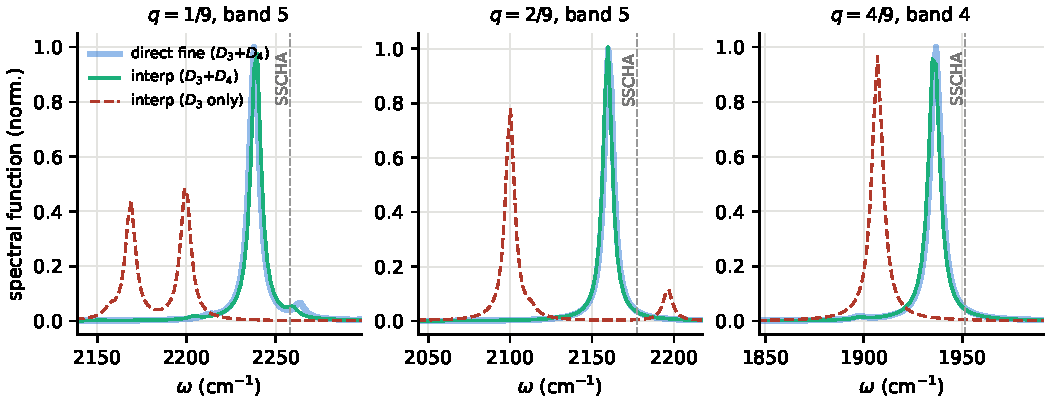
\includegraphics[width=\linewidth]{figs/d4_spectral.pdf}
\caption{One-phonon spectral functions in a $D_4$-dominated regime
($g_3=0.15$, $g_4=2.0$) at interpolated wavevectors of the $(1,1,9)$ mesh.
Blue: direct fine-mesh TDSCHA Lanczos ($D_3{+}D_4$). Aqua: interpolated
from the coarse $(1,1,3)$ ensemble ($D_3{+}D_4$) --- it overlays the direct
reference. Red dashed: the same interpolation with the fourth order dropped
($D_3$ only), displaced by the quartic hardening of $30\dots56\,\si{cm^{-1}}$.
The SSCHA frequency is marked; curves normalized to the direct peak.}
\label{fig:d4spectral}
\end{figure}

\subsection{Atomic centering of the four-phonon vertex}
\label{sec:d4center}

The SnTe tests show where the simple D4 treatment fails.  In the
underresolved $L=2$ real-material cells of Sec.~\ref{sec:atomic}, the
plain-window $D_4$ pass has the same basis-tie ambiguity that broke the
plain $D_3$ estimator.  A low-symmetry benchmark on the SnTe force field
(R3m phase at
$T=\SI{180}{K}$, where the free-energy Hessian requires the fourth order:
the $A_1$ order-parameter mode is $76.2 \to 25.3\,\si{cm^{-1}}$ with the
$D_3$ bubble alone and $\to 39.1\,\si{cm^{-1}}$ with $D_4$) showed that the
$2{\times}2{\times}2 \to 4{\times}4{\times}4$ interpolation with plain
$D_4$ systematically \emph{under-captures} the $D_4$ renormalization of
the spectral first moment: at $N=4000$ the direct fine-mesh $D_4$ shift of
$\langle\omega\rangle$ is $-22.9\,\si{cm^{-1}}$ but the interpolation
recovers only $-14.8\,\si{cm^{-1}}$ (64\%), while the $D_3$-only moments
agree to $\sim\SI{5}{cm^{-1}}$ --- the deficit is $D_4$-specific.

The difficulty is structural.  The mathematical vertex has four logical
legs, $\Phi^{(4)}(E_w,E_v,I_w,I_v)$: two external two-phonon legs and two
internal legs contracted with the two-phonon vector.  The existing Julia
estimator stores only two pair-slot field families, $w$ and $v$, and reuses
them for both internal and external legs.  Any D4 centering that manipulates
only these two slots is therefore a projection of a four-leg geometry onto a
two-slot implementation.

Two such projections were tested.  The first is the \texttt{reference} mode.
It runs the D4 term on the channel-0 atomic passes: all four D4 legs carry
the same atom-resolved window $W_{a,o}$ relative to an external pinned atom.
This mode is tensor-free, permutation-symmetric, ASR-safe under the existing
q-space projector, and exactly equal to plain D4 at commensurate q.  But the
pinned atom is not one of the four D4 vertex legs, so the centering reference
is physically wrong.

What the external-reference scheme does \emph{not} get right is the
centering reference: the pinned atom is not one of the four vertex legs, so
all four legs are imaged relative to an external point and every leg
suffers the $L{=}2$ tie dilution, compounded over the four-fold product.
Consistently, on the R3m benchmark the centered $D_4$ vertex block differs
from the plain one by 78\% in norm, yet the $A_1$ observable barely moves
($-5.6$ vs $-6.1\,\si{cm^{-1}}$, both far from the direct $-16.1$ at
$N=1000$).

The second projection is \texttt{d4\_center="leg"}.  It is the direct
analogue of the D3 force-channel construction: pin the D4 leg that carries
the force.  Across the estimator terms the force leg
occupies all four positions: the two external legs through the
$y_w(q_1)\,f_Y x_v(q_2)$ and $f_Y x_w(q_1)\,y_v(q_2)$ parts of the
$\langle xx\alpha\rangle$-type term, and the two internal ones through the
$f_\psi$-contracted term ($\overline{\alpha_1 x^*_v}\,f_\psi\,y^*_w$ and
its $w\!\leftrightarrow\!v$ mirror).  Splitting the kernel by these four
force positions (channel gates \texttt{d4\_force\_ew/ev/iw/iv}, the $D_4$
analogue of the $D_3$ $1/3{+}2/3$ split) reveals a decisive
simplification: within each channel the pinned delta touches only the
\emph{force} ($Y$) field of one slot, while the displacement ($X$) field
of the same slot always belongs to the other, windowed legs.  The
centering is therefore realized without any new field family, by passing
per slot the $X$ field of the atomic window $W_{a,o}$ and the $Y$ field of
the pinned delta: one $W$-force call (channels $ew{+}iw$, $Y_w=\delta$)
and one $V$-force call ($ev{+}iv$, $Y_v=\delta$) per pinned atom/origin,
i.e.\ $2\,n_{\mathrm{at}}N_c$ extra kernel calls and zero new field sets.
Because every gated term is linear in the delta-carrying $Y$ field, the
sum over pinned atoms and full coarse origins reconstructs the force-leg
atom sum with no prefactor, and at commensurate $q$ it collapses to the
plain $D_4$ estimator configuration by configuration.  The summed
four-channel kernel $\sum_{\ell}\delta(\ell)\,W\!\otimes\!W\!\otimes\!W$
is symmetric under leg exchange, so the $4$-leg permutation symmetry of
$\Phi^{(4)}$ is preserved exactly, as for $D_3$; the channel split and the
commensurate identity are locked by unit tests
(\texttt{test\_d4\_center.py}).

This construction passes the algebraic tests: the channel split reproduces
the all-channel D4 call, the commensurate identity holds, and the summed
four-channel kernel is formally symmetric.  But the SnTe spectra show that
these identities are necessary, not sufficient.  The first
complete Fm-$\bar 3$m smoke benchmark with all three $D_4$ modes
($T=\SI{280}{K}$, quartic couplings scaled by $3$, $N=300$, 25 Lanczos
steps) gives a direct spectral-moment $D_4$ shift of
$-7.25\,\si{cm^{-1}}$.  Plain $D_4$ captures only
$-1.65\,\si{cm^{-1}}$ (23\%), the external-reference centering improves to
$-3.63\,\si{cm^{-1}}$ (50\%), but the pin-force-leg construction gives the
\emph{wrong sign}, $+2.05\,\si{cm^{-1}}$ (-28\% capture) and the worst
line-shape distance.  A larger, cleaner partially completed run
($T=\SI{280}{K}$, $p_4{\times}2$, $p_3{\times}1.6$, $N=2000$, first
off-grid shell) confirms that the residual error is mode dependent rather
than a scalar normalization: for band 5, plain $D_4$ captures
$+5.93/+8.71=68\%$ of the direct first-moment shift, whereas for band 0 it
slightly overshoots, $+1.48/+1.33=111\%$.  At the physical $T=\SI{400}{K}$
couplings the total shift is too small to be decisive, but the completed
part of the run again shows only partial capture (plain 14\%, reference
41\%).  The current conclusion is therefore negative: the implemented
\texttt{d4\_center="leg"} split preserves channel sums and the
commensurate limit, but it does not yet realize the physically correct
four-leg minimal-image interpolation.  The next diagnostic must compare the
four force channels at the operator level against an explicit geometry-only
four-leg target before using longer production spectra as evidence.
The geometry diagnostic makes the failure concrete.  A single $w$ or $v$
window simultaneously represents an external leg and an internal leg at
different momenta.  Pinning only the force field does not independently
center the other three D4 legs.
As a safety patch, the boolean production switch
\texttt{d4\_center=True} has been changed back to the legacy
external-reference mode; the failed pin-force-leg construction remains
available only as the explicit diagnostic option
\texttt{d4\_center="leg"}.  This avoids silently selecting the wrong-sign
scheme while the true four-leg centering target is unresolved.  The patch
is verified in the SnTe environment by running with the branch overlay
\texttt{PYTHONPATH=/tmp/tdscha\_pyshim}: a D4-only operator application at
the first off-grid shell gives relative difference $0.0$ between
\texttt{d4\_center=True} and \texttt{d4\_center="reference"}.  Without this
overlay, \texttt{micromamba run -n sscha} imports the installed
site-package copy of TDSCHA and does not exercise the working tree.  A
pure geometry scan on the SnTe $L=2$ cell gives the immediate reason:
comparing the current force-star image
assignment with a true four-leg perimeter target over all 8192 atom/cell
classes (nearest image shell) gives total-variation distance mean 0.614,
maximum 1.0, and nonzero mismatch in 85.3\% of cases.  Thus the problem is
not the q-space ASR projector (which gives the same behavior with
\texttt{atomic} and \texttt{atomic\_delta}), but the geometry target
itself: the force-star product is not a faithful four-leg centering rule.
The word ``reference'' in \texttt{d4\_center="reference"} should therefore
not be read as a stored-$\Phi^{(4)}$ oracle.  That mode remains tensor-free:
it reuses the channel-0 atom/origin stochastic passes and applies the same
atom-resolved window to the D4 legs relative to an external pinned atom,
averaging over pinned atoms and origins.  The pinned atom is not one of the
four D4 vertex legs, so this is a legacy comparison/guardrail rather than the
correct four-leg centering.  In the branch-overlay SnTe smoke benchmark
(\texttt{PYTHONPATH=/tmp/tdscha\_pyshim}, $N=300$, 25 Lanczos steps,
quartic scale $3$), the direct D4 first-moment shift is
$-7.25\,\si{cm^{-1}}$ while reference mode gives
$-3.63\,\si{cm^{-1}}$ (50\% capture, normalized $L^1=0.391$ against the
direct $D_3{+}D_4$ spectrum).

\paragraph{Restarting from a four-leg target.}
The replacement design is to lift the stochastic $D_4$ interpolation from
the two reused pair slots to the four logical legs of the
two-phonon-to-two-phonon vertex: the external legs $(E_w,E_v)$ and the
internal legs $(I_w,I_v)$ contracted with the two-phonon vector.  On the
atom-resolved extended lattice one first builds a purely geometric target
$T_4(E_w,E_v,I_w,I_v)$ by assigning the periodic images of the four atoms
that minimize a symmetric cluster cost, for example the complete-graph sum
of squared pair distances, with exact tie splitting.  This target is then
projected onto the linear subspace that enforces the three invariants
required of the estimator: the 24 four-leg permutations, unit folded class
sums on every commensurate image class (so the coarse-grid operator is
exactly the current plain $D_4$ operator), and translational acoustic sum
rules on every leg.  This step still uses only geometry and linear algebra;
no entry of $\Phi^{(4)}$ is formed, stored or fitted.

The projected target is not meant to be evaluated as a dense four-index
object.  Instead it should be factorized once into a small separable sum
\begin{equation}
T_4^{\mathrm{ASR}} \simeq \sum_{r=1}^{R_4} c_r\,
A_r(E_w)\,B_r(E_v)\,C_r(I_w)\,D_r(I_v),
\label{eq:d4factor}
\end{equation}
with atom-resolved one-leg factors whose folded class sums satisfy the same
partition and ASR constraints.  The runtime implementation is then a
slot-lifted $D_4$ kernel, selected by a new explicit mode such as
\texttt{d4\_center="factor4"}, which accepts four logical D4 field slots
rather than reusing the same $w,v$ arrays for both internal and external
legs.  Each rank term is one batched D4 pass over the existing $O(N_f)$
pair list, so the cost is
$O(R_4\,N_{\mathrm{conf}}\,N_{\mathrm{sym}}\,N_f\,n_b^2)$ and remains
linear in the interpolation mesh as long as the factor rank $R_4$ is fixed
by the coarse-cell geometry rather than by $N_f$.  The validation gate is
ordered accordingly: pure SnTe $L=2$ geometry (where the old force-star
target must fail), exact commensurate operator identity, Hermiticity,
acoustic-leg scaling, toy-model rank convergence, and only then the
Fm-$\bar 3$m first-off-grid-shell SnTe benchmark with the plain,
reference and leg modes kept as negative controls.

\paragraph{Equivalence: this is not a low-rank fit of $\Phi^{(4)}$.}
The object being factorized in Eq.~\eqref{eq:d4factor} is the
\emph{image-assignment kernel}, not the fourth-order force constant.  The
proof is the same kernel argument as Sec.~\ref{sec:kernel}, now with four
logical slots.  Collapse atom and Cartesian indices into $a$ and let
$i=(a,\Rv)$ denote an atom in one folded coarse supercell.  For one ordered
$D_4$ channel take four logical fields $z_\ell(i)$, with one of them the
force field $y$ and the other three displacement fields $x$ (the four force
positions are summed afterward).  A rank-$r$ windowed field is
\begin{equation}
Z_{\ell r}(\qv_\ell)
 = \frac{1}{\sqrt{\Nc}}\sum_i
 W_{\ell r}(i;\qv_\ell)\,
 e^{-i\qv_\ell\cdot \Rv_i}\,z_\ell(i),
\qquad \ell=1,\ldots,4 .
\label{eq:d4windowfield}
\end{equation}
The rank-$r$ contribution to the stochastic estimator is the same four-field
product already evaluated by the q-space Lanczos kernel,
\begin{equation}
\widehat C^{(r)}_4(\qv_1,\qv_2,\qv_3,\qv_4)
 = \bigl\langle
 Z_{1r}(\qv_1)Z_{2r}(\qv_2)Z_{3r}(\qv_3)Z_{4r}(\qv_4)
 \bigr\rangle .
\end{equation}
By multilinearity,
\begin{equation}
\sum_r c_r \widehat C^{(r)}_4
=\frac{1}{\Nc^2}\sum_{i_1i_2i_3i_4}
K_R(i_1,i_2,i_3,i_4;\qv_1,\ldots,\qv_4)
e^{-i\sum_\ell \qv_\ell\cdot\Rv_{i_\ell}}
\bigl\langle z_1(i_1)z_2(i_2)z_3(i_3)z_4(i_4)\bigr\rangle ,
\label{eq:d4kernelaverage}
\end{equation}
where
\begin{equation}
K_R=\sum_r c_r
W_{1r}(i_1;\qv_1)W_{2r}(i_2;\qv_2)
W_{3r}(i_3;\qv_3)W_{4r}(i_4;\qv_4)
\end{equation}
is the factorized geometry kernel.  Thus the factorization changes only the
real-space image weights multiplying the same stochastic four-field
average.  It is not a decomposition, compression, or fit of
$\Phi^{(4)}$.

At SSCHA stationarity, Gaussian integration by parts gives for a force leg
in slot 4
\begin{equation}
\bigl\langle x_1 x_2 x_3 y_4 \bigr\rangle
= -\,G_1G_2G_3\,
\left\langle
\frac{\partial^4 V}{\partial u_1\partial u_2\partial u_3\partial u_4}
\right\rangle ,
\label{eq:d4ibp}
\end{equation}
up to the disconnected pieces proportional to
$\langle u\otimes\delta f\rangle$, which vanish when the SSCHA auxiliary
matrix is converged.  The pre-filtering factors of
Sec.~\ref{sec:prefilter} cancel the propagators $G_\ell$ exactly as in the
$D_3$ derivation.  Therefore Eq.~\eqref{eq:d4kernelaverage} is, in the
infinite-sampling limit, precisely the q-space contraction of the
fourth-order vertex interpolated with the kernel $K_R$.  If
$K_R=T_4^{\mathrm{ASR}}$ exactly, the stochastic estimator is equivalent to
forming a centered and ASR-projected $\Phi^{(4)}$ with that same geometry
target and contracting it with the two-phonon vector; the implementation
simply performs the contraction before any tensor is ever materialized.
If the factor rank is finite, the only deterministic error is the kernel
error $K_R-T_4^{\mathrm{ASR}}$, not an uncontrolled fit to force constants.

\paragraph{Exact identity at commensurate q.}
The commensurate proof is independent of the force field.  Let
$[i]$ denote an atom/cell class modulo the coarse supercell, and let
$i+nL$ denote any extended image of that class.  For commensurate
wavevectors $\qv_\ell$ of the coarse mesh,
$e^{-i\qv_\ell\cdot(\Rv_i+nL)}=e^{-i\qv_\ell\cdot\Rv_i}$, and the
periodic configuration has $z_\ell(i+nL)=z_\ell(i)$.  If the projected
kernel satisfies the partition constraint
\begin{equation}
\sum_{n_1n_2n_3n_4}
K_R(i_1+n_1L,i_2+n_2L,i_3+n_3L,i_4+n_4L)=1
\label{eq:d4partition}
\end{equation}
for every folded quadruple $([i_1],[i_2],[i_3],[i_4])$, then regrouping
Eq.~\eqref{eq:d4kernelaverage} by folded classes gives
\begin{align}
\sum_{\{n_\ell\}}&
K_R(i_1+n_1L,\ldots,i_4+n_4L)
e^{-i\sum_\ell\qv_\ell\cdot(\Rv_{i_\ell}+n_\ell L)}
\prod_\ell z_\ell(i_\ell+n_\ell L)
\nonumber\\
&=
e^{-i\sum_\ell\qv_\ell\cdot\Rv_{i_\ell}}
\prod_\ell z_\ell(i_\ell),
\end{align}
which is exactly the unwindowed coarse-supercell stochastic product.  This
holds configuration by configuration and for arbitrary displacements,
forces and Lanczos vector $\alpha_1$; no ensemble average and no
properties of $\Phi^{(4)}$ are used.  Consequently any factorized
four-leg window satisfying Eq.~\eqref{eq:d4partition} reproduces the
current plain $D_4$ q-space operator exactly at all commensurate
wavevectors.  The ASR and permutation projections can change the off-grid
image assignment only inside the null space of this partition constraint.

\paragraph{Tensor-free fitting of the kernel.}
The fit of Eq.~\eqref{eq:d4factor} can also be performed without building a
dense fourth-rank target array.  What is needed by constrained ALS or a
randomized CP fit are contractions of the target with three one-leg
vectors, for example
\begin{equation}
\mathcal F_T[p,q,r](i_1)
 = \sum_{i_2i_3i_4}
T_4^{\mathrm{ASR}}(i_1,i_2,i_3,i_4)\,
p(i_2)q(i_3)r(i_4).
\label{eq:d4targetforce}
\end{equation}
This is exactly the geometry analogue of contracting three displacement
legs of $\Phi^{(4)}$ to obtain a force-like object on the remaining leg,
but the contraction uses only the image-assignment oracle $T_4$ and the
linear ASR/partition/permutation projectors.  The oracle returns the
minimal four-leg image weights and tie splits for a requested quadruple;
the projected contraction can be applied matrix-free by composing this
oracle with the constraint projectors.  The ALS normal equations, or a
randomized objective based on probes
$\langle a\otimes b\otimes c\otimes d,\,T_4^{\mathrm{ASR}}-K_R\rangle$,
therefore require only target contractions such as
Eq.~\eqref{eq:d4targetforce}.  Neither the force-constant tensor
$\Phi^{(4)}$ nor even a dense stored $T_4$ is required.  The stored runtime
data are only the one-leg factors and coefficients entering
Eq.~\eqref{eq:d4factor}.

\paragraph{Choosing a clean SnTe benchmark.}
The R3m SnTe benchmark is physically relevant but technically awkward:
the interpolated fine mesh contains imaginary modes, and masking them can
obscure the D4 interpolation error.  The quantitative benchmark was
therefore moved to the cubic Fm-$\bar 3$m phase, where the auxiliary
dynamical matrix interpolates cleanly from $2^3$ to $4^3$ and the q-space
Lanczos does not need symmetry post-processing.

The D4 signal must be made large enough to measure, but this cannot be done
by simply multiplying the quartic force constants.  If the quartic
couplings are scaled and the SSCHA minimum is recomputed, the quartic
tadpole is resummed into the auxiliary dynamical matrix: the $\Gamma$ TO
auxiliary frequency hardens from $54$ to $86\,\si{cm^{-1}}$, fluctuations
are suppressed, and the residual D4 Hessian shift shrinks to
$+1.1\,\si{cm^{-1}}$.  A large D4 signal obtained without re-minimizing is
therefore an artifact of violating the SSCHA stationarity condition.

The useful knob is the cubic coupling.  In the cubic phase, parity makes
the SSCHA minimum independent of $d_3$, so $d_3$ can be scanned without
re-minimization.  The D4 response diagrams visible in the two-phonon sector
scale as $d_3^2d_4$, while the auxiliary loop does not carry $d_3$.  At the
$2p_4$ minimum the measured scan gives
$\Sigma_{\mathrm{bubble}}=1883s^2$ and
$\Sigma_{D_4}=172s^2\,\si{cm^{-2}}$ for $p_3\to s\,p_3$.  The benchmark
therefore uses the first off-grid shell of the $4^3$ mesh, where the upper
optical branch has a stable static response and a sizeable D4
$w_{\mathrm{eff}}$ shift, about $35.2\to53.1\,\si{cm^{-1}}$ in the direct
fine calculation.

\subsection{Fourth order in the atom-centred Fourier gauge: the four-leg
problem that factorizes}
\label{sec:d4-atom-fourier}

The real-space centering attempts above (\texttt{leg}, \texttt{reference},
and the factor-4 program) all struggle with the same obstruction: the
minimal-image assignment of a four-atom cluster is a genuine four-body
geometry problem that does not split into pairs.  There is, however, one
regime in which it \emph{does} split exactly, and it is the same
observation that fixed the third order in Sec.~\ref{sec:atom-fourier}:
move the atom phase into the Fourier transform (the
\texttt{atom\_fourier=True} kernel $P_{ab}(\qv,\kv)$ of
Eq.~\eqref{eq:atom-fourier-kernel}) and interpolate the resulting
non-periodic Bloch field.

The reason is a momentum count.  The $D_4$ term maps the incoming
two-phonon block at the internal pair $(\qv',Q-\qv')$ onto the outgoing
block at $(\qv,Q-\qv)$.  Because the estimator contracts the incoming
block with \emph{conjugated} Bloch fields, the four vertex legs carry the
momenta $(+\qv,-\qv,-\qv',+\qv')$.  Pinning the first leg to the home cell
and using translational invariance,
\begin{equation}
V(\qv,\qv')_{abcd}
= \sum_{\Rv_2\Rv_3\Rv_4}
\Phi^{(4)}(a\mathbf 0,b\Rv_2,c\Rv_3,d\Rv_4)\,
e^{2\pi i[\qv\cdot\Rv_2+\qv'\cdot(\Rv_3-\Rv_4)]} .
\label{eq:d4-two-momenta}
\end{equation}
The two \emph{independent} internal momenta $\qv$ and $\qv'$ each couple to
exactly one pair offset: $\qv$ to $\Rv_2$ (minimal image near
$\boldsymbol\tau_a-\boldsymbol\tau_b$) and $\qv'$ to $\Rv_3-\Rv_4$
(minimal image near
$-(\boldsymbol\tau_c-\boldsymbol\tau_d)$).  These are precisely the harmonics continued by
$P_{ab}(\qv,\kv)$ on the outgoing leg pair and by
$\overline{P_{cd}(\qv',\kv')}$ on the incoming pair.  The correct four-leg
continuation is therefore the \emph{tensor product of the pairwise
atom-centred kernel with itself} --- which is exactly what the existing
fold/unfold applies, with $P_{ab}$ on the unfold and its conjugate on the
fold.  No new geometry, no four-body image search, and no new code path are
needed: the class already routes $D_4$ through the correct map whenever
\texttt{atom\_fourier=True}.

This is not in contradiction with the four-body difficulty of
Sec.~\ref{sec:d4center}.  What factorizes is the \emph{q-space}
interpolation of the two-phonon-to-two-phonon vertex, whose two internal
momenta are independent by construction.  The residual real-space content
--- which lattice image each pair harmonic belongs to --- is the same
pairwise minimal-image question already solved for $D_3$, applied once per
momentum.

\paragraph{Noise-free vertex verification.}
The quartic vertex of the anharmonic diatomic chain is known in closed
form ($6g_4(\boldsymbol\delta_i-\boldsymbol\delta_j)^{\otimes4}$ per bond and Cartesian
component), so the interpolation map is testable with zero stochastic
noise.  Sampling the exact vertex at the coarse pairs, applying the
production kernel, and comparing against the exact fine vertex over all
$(\qv,\qv')$ pairs gives
(\texttt{report/interpolation/scripts/d4\_atom\_fourier\_oracle.py}):
\begin{center}
\small
\begin{tabular}{lcc}
\toprule
coarse $\to$ fine & atom-centred Fourier & trilinear (off-grid) \\
\midrule
$3\to9$ & $1.4\times10^{-31}$ & $5.6\times10^{-2}$ \\
$2\to4$ & $8.7\times10^{-33}$ & $1.8\times10^{-1}$ \\
$2\to6$ & $3.1\times10^{-32}$ & $1.8\times10^{-1}$ \\
$4\to8$ & $4.3\times10^{-32}$ & $1.9\times10^{-2}$ \\
\bottomrule
\end{tabular}
\end{center}
The atom-centred Fourier continuation reconstructs the exact four-leg
vertex to machine zero, including the $L=2$ case in which every off-grid
pair is a Nyquist tie split $50/50$; that the $L=2$ result is exact also
independently confirms the sign/branch convention of
Eq.~\eqref{eq:d4-two-momenta}, since a single wrong sign would destroy the
cancellation.  Adding a second-neighbour quartic bond (harmonics at
$|\Rv|=2$) makes the map exact on the meshes that resolve it
($4\to8$, $5\to10$: rel.\ error$^2<10^{-31}$) and honestly aliased on the
one that does not ($2\to4$: rel.\ error$^2=0.25$).  The limit is
therefore the coarse mesh's real-space range, exactly as for $D_3$ one
order down --- not a defect of the continuation.

\paragraph{Operator-level tests.}
The shipped code path is covered by
\texttt{tests/test\_trilinear/test\_d4\_atom\_fourier.py}: exact
reconstruction of the closed-form vertex; the three independent leg
exchanges of $\Phi^{(4)}$ (via the kernel mirror identity
$P_{ab}(\qv,\kv)=P_{ba}(-\qv,-\kv)$ and at the vertex level); preservation
of the acoustic sum rule on all four legs, with deliberately broken
non-cardinal and atom-pinned control maps confirming the test has teeth;
Hermiticity of the isolated $D_4$ two-phonon block at time-reversal
invariant and generic coarse $Q$; the unfold mirror
$D(Q-\qv)=D(\qv)^T$; and the commensurate identity to the parent
\texttt{QSpaceLanczos} with $D_4$ shown to be non-vacuously active.  The
ASR test rests on two facts the kernel supplies and a pinned-window map
does not: $P_{ab}$ is independent of the atoms of the other pair (so the
sum rule on the non-interpolated legs survives), and it is exactly cardinal
at $\Gamma$ (where the moving-pair sum rule lives).

\paragraph{Spectral benchmark.}
Figure~\ref{fig:d4atomfourier} and the table below compare the two q-space
schemes against a direct fine-mesh reference from an independent $(1,1,9)$
ensemble of the same chain, in the $D_4$-dominated regime of
Sec.~\ref{sec:d4} ($g_3=0.15$, $g_4=2.0$, $N_I=6000$, $110$ Lanczos
steps).  Because this class refines the internal loop $\qv'$ and keeps the
external $Q$ on the coarse mesh, the probes are coarse $Q$ and the
interpolation gain is a better-resolved two-phonon continuum --- exactly
the SnTe $\Gamma$-TO setup.  The metric is the $D_4$-induced peak shift,
i.e.\ the renormalization, not the absolute frequency.
\begin{center}
\small
\begin{tabular}{lccccc}
\toprule
probe & direct $D_4$ shift & \multicolumn{2}{c}{atom Fourier} &
\multicolumn{2}{c}{trilinear} \\
\cmidrule(lr){3-4}\cmidrule(lr){5-6}
& (\si{cm^{-1}}) & capture & $L_1$ & capture & $L_1$ \\
\midrule
$\Gamma$, band 5 & $+52.9\pm1.9$ & $109\%$ & $0.38$ & $72\%$ & $0.67$ \\
$\Gamma$, band 4 & $+14.7\pm3.7$ & $139\%$ & $0.80$ & $-16\%$ & $0.51$ \\
$q{=}3/9$, band 5 & $+22.6\pm1.8$ & $112\%$ & $0.37$ & $90\%$ & $0.35$ \\
$q{=}3/9$, band 4 & $+21.0\pm4.7$ & $89\%$ & $0.21$ & $61\%$ & $0.41$ \\
\bottomrule
\end{tabular}
\end{center}
The error bars are the seed-to-seed spread of the direct $D_4$ shift over
three independent fine ensembles
(\texttt{d4\_seed\_noise\_control.py}).  The atom-centred Fourier scheme
captures the fourth-order renormalization to within the stochastic noise
floor at every probe, whereas piecewise-trilinear corners systematically
under-capture and, for the weak-signal $\Gamma$ band-4 line, even return
the wrong sign --- the four-leg analogue of the $D_3$ hardening of
Sec.~\ref{sec:atomic}.  The remaining atom-Fourier deviations
($\lesssim1\times$ the noise) are consistent with sampling, not with a
systematic interpolation bias.

\begin{figure}[t]
\centering
\includegraphics[width=\linewidth]{figs/d4_atom_fourier.pdf}
\caption{Fourth-order fitting quality in q space.  (a)~A representative
Cartesian element of the exact four-leg quartic vertex of the chain along a
Brillouin-zone crossing (blue), reconstructed from the coarse samples
(open circles) by the atom-centred Fourier kernel (green, on top of the
exact curve) and by piecewise-trilinear corners (orange, chords).
(b)~Spectral function at $\Gamma$ (band~5) in the $D_4$-dominated regime;
the dotted grey line is the $D_3$-only continuum before the quartic shift.
(c)~Fraction of the direct fourth-order peak shift recovered by each
scheme at four probes; grey bands are the stochastic noise floor from
three-seed direct references.  The atom-centred Fourier continuation lands
inside the noise band everywhere; trilinear corners under-capture and flip
sign for the weakest line.}
\label{fig:d4atomfourier}
\end{figure}

The practical conclusion is that the fourth order needs no separate
solution on SnTe-like cells: the atom-centred Fourier gauge that repairs
$D_3$ repairs $D_4$ by the same mechanism, because in q space the two
internal momenta of the two-phonon vertex are independent and the
minimal-image assignment factorizes into two pairwise problems.  The
real-space four-leg centering program of Sec.~\ref{sec:d4center} remains
the route for observables that genuinely couple all four legs at once
(for instance an external $Q$ that is itself interpolated), but it is not
required for the interpolated spectral functions studied here.

\subsection{Production case: CsSnI$_3$ Raman, $4^3\to8^3$}
\label{sec:cssni3}

The largest test is a full anharmonic Raman spectrum of the hybrid
perovskite CsSnI$_3$ in its P4/mbm phase at $T=\SI{500}{K}$: a ten-atom cell
(30 bands), a $4\times4\times4$ supercell (640 atoms), and a converged SSCHA
ensemble subsampled to $N=1500$ configurations.  The unpolarized spectrum
($45I_0+7\sum_{i=1}^{6}I_i$, continued-fraction Green function, 100 Lanczos
steps, $D_3{+}D_4$) is computed natively on the $4^3$ mesh and by
interpolating the internal two-phonon loop to $8^3$ with
\texttt{atom\_fourier}.  Since the Raman perturbation sits at $\Gamma$, on
the coarse mesh, the interpolation refines the two-phonon continuum while
reusing the coarse stochastic kernel.

\paragraph{A calibration lesson.}  A first attempt produced a large apparent
mesh effect --- a single native band near $\SI{90}{cm^{-1}}$ moving to
$125$--$\SI{155}{cm^{-1}}$ at $8^3$.  That was an artifact of an
\emph{ensemble-initialization bug} in the driver script, not of the method:
after subsampling the ensemble with \texttt{Ensemble.split} one must call
\texttt{ensemble.init()} to refresh the q-space forces (otherwise
\texttt{QSpaceLanczos} reuses stale \texttt{forces\_qspace}, because it only
recomputes them when \texttt{u\_disps\_qspace} is absent), and the ensemble
must be built around the generation dynamical matrix and reweighted to the
converged one with \texttt{update\_weights}, exactly as
\texttt{load\_distributed\_tdscha} does.  With the uninitialized ensemble the
tridiagonal coefficients were $\sim\!100\times$ too large and the line shape
became sensitive to the step count.  Once the ensemble is initialized
correctly the spectrum is stable: the unpolarized peak is
$\SI{33.1}{cm^{-1}}$ at $40$, $60$, $80$ and $100$ Lanczos steps
identically.  (For this soft, strongly anharmonic system the raw
coefficients still grow geometrically, $b_nc_n\!\sim\!10^{24}$ by step 100,
but the terminated continued fraction is numerically insensitive to this ---
the spectrum does not move --- so the growth is benign.)

\paragraph{Result.}  Figure~\ref{fig:cssni3} shows the corrected spectrum.
It is \emph{soft-mode dominated}, peaking near $\SI{33}{cm^{-1}}$ with a weak
optical band near $\SI{93}{cm^{-1}}$, consistent with the octahedral-tilt
central peak expected for this material near its transition, and consistent
with the user's independent production run.  The native $4^3$ and
interpolated $8^3$ spectra \emph{agree}: their normalized $L_1$ distance is
$0.0012$ and the optical band sits at $\SI{93}{cm^{-1}}$ in both.  Physically
this is expected --- the dominant signal is the one-phonon soft mode, whose
$\Gamma$ frequency is pinned identically on both meshes and which is
insensitive to the internal two-phonon mesh --- and it is the correct
outcome: the interpolation faithfully reproduces the native calculation
rather than distorting it.

\paragraph{What was learned.}  Two things.  First, the incommensurate points
carry their full anharmonic weight: a direct probe of the interpolated
two-phonon coupling magnitude gives an off-grid/commensurate ratio of
$1.00$, so there is no loss of anharmonic strength at the interpolated
wavevectors (the concern that motivated this test).  Second, the cost of the
refinement is almost nothing: the native $4^3$ run took \SI{3884}{s} and the
interpolated $8^3$ run \SI{4085}{s} plus a one-time \SI{45}{s} construction
--- only $5\%$ more wall time for eight times as many internal momenta,
because the expensive stochastic kernel runs on the 64 coarse pairs in both
and the interpolation adds only the fold/unfold ($\sim\!\SI{0.3}{s}$ per step
against $\sim\!\SI{5.5}{s}$ for the kernel).  A native $8^3$ calculation would
instead need an independent $8^3$ ensemble and about eight times more kernel
pairs per step.  The fold/unfold were optimised to \texttt{einsum}
contractions on the atom-block kernel, and the kernel build to a per-pair
matrix product using the phase factorisation
$e^{2\pi i(\qv-\mathbf x)\cdot\mathbf R}
=e^{2\pi i\qv\cdot\mathbf R}\,\overline{e^{2\pi i\mathbf x\cdot\mathbf R}}$.
The saved Lanczos coefficients (\texttt{save\_abc}) let the spectra be
replotted at any smearing or grid without repeating the multi-hour run.

\begin{figure}[t]
\centering
\includegraphics[width=\linewidth]{figs/cssni3_raman_interp.pdf}
\caption{CsSnI$_3$ P4/mbm unpolarized Raman at $T=\SI{500}{K}$
($D_3{+}D_4$, $N=1500$, 100 Lanczos steps).  Blue: native $4^3$ q-space
TDSCHA Lanczos.  Green: the same observable with the internal two-phonon
loop interpolated to $8^3$ (\texttt{atom\_fourier}).  (a)~absolute;
(b)~area-normalized.  The spectrum is soft-mode dominated
($\sim\SI{33}{cm^{-1}}$) and the two meshes agree to a normalized $L_1$ of
$0.0012$: the interpolation faithfully reproduces the native result at $5\%$
extra wall time.  (The large shift seen before correcting an
ensemble-initialization bug in the driver was an artifact, not physics.)}
\label{fig:cssni3}
\end{figure}

%======================================================================
\section{Comparison with other anharmonic codes and a recommendation}
\label{sec:codes}

Every method in this report was validated against the centered-tensor
oracle, i.e.\ the standard \texttt{cellconstructor} pipeline.  This
section places that choice in context: how the established anharmonic
codes interpolate three- and four-phonon interactions, which of their
design decisions reappear here in tensor-free form, and which of the
three interpolation strategies implemented on this branch we recommend.
A short verification note first.  The fold/unfold implementation
(\texttt{QSpaceTrilinearLanczos}, including the atom-centred cardinal
kernel of Eq.~\eqref{eq:atom-fourier-kernel}) passes its sixteen unit
tests: exact commensurate identity against \texttt{QSpaceLanczos},
Hermiticity (unfold $=$ adjoint of fold), pair-transpose symmetry
$A(Q-k)=A(k)^{T}$, corner geometry, and the cardinal-kernel identities
(\texttt{tests/test\_trilinear/}).  Independently of that suite we
re-derived the one-dimensional atom-centred cardinal kernel on the SnTe
example $V(q)=A(e^{2\pi i q}-1)$ of Sec.~\ref{sec:atom-fourier}: with
$N=2$ coarse samples and $d=\tau_{\mathrm{Te}}-\tau_{\mathrm{Sn}}=1/2$ the
kernel is the identity at commensurate $q$ to machine precision and
reconstructs the sine envelope exactly at $q=1/4$ ($|V|=\sqrt2\,|A|$,
phase error $0$), while the trilinear tent gives $|A|$.  The code
implements the equation.

\subsection{Two families, one principle: a compact real-space
representation}
\label{sec:codes-families}

All production codes that need three-phonon vertices on a dense $q$ mesh
evaluate them as the \emph{exact Fourier transform of a localized
real-space object}.  They differ only in how that object is built.

\paragraph{(a) Real-space supercell codes.}  In this family the
third-order force constants are built directly in the supercell.  In
phono3py \cite{phono3py,phono3py2015} they are constructed from finite
displacement pairs (or fitted with
\texttt{symfc}/ALM), stored compactly with the first atom pinned in the
home primitive cell, and truncated with a pair cutoff
(\texttt{--cutoff-pair}): any triplet whose interatomic distances exceed
the cutoff is exactly zero.  ShengBTE's \texttt{thirdorder.py}
\cite{shengbte} does the same with a cutoff expressed as an $n$-th
nearest-neighbour shell; ALAMODE \cite{alamode} and TDEP \cite{tdep} fit
the same kind of compact real-space tensor from molecular-dynamics data
by (constrained) least squares.  The image assignment is therefore made
\emph{by construction}: only short-range, minimal-distance triplets
exist, and the vertex at any $\qv$ is the exact transform
$V\propto\sum\Phi^{(3)}_{abc}\,e^{i\qv_1\cdot\mathbf r_a+
i\qv_2\cdot\mathbf r_b+i\qv_3\cdot\mathbf r_c}$ evaluated on the target
mesh.  No $q$-space interpolation of vertex samples is ever performed.
Acoustic sum rules are imposed on the stored tensor, either by drift
removal plus index-exchange averaging (phono3py's
\texttt{--fc-symmetry}), by an iterative least-squares compensation
(ShengBTE), or exactly inside the fitted basis (\texttt{symfc}, ALAMODE).
One detail is worth singling out: since v3, phono3py averages the
real-to-reciprocal transform over the three equivalent choices of the
pinned atom (\texttt{make\_r0\_average}), keeping only shortest-vector
triplets through a multiplicity mask (\texttt{all\_shortest}).  This is
an atom-resolved pinning with tie handling --- conceptually the closest
relative of the pinned windows of Sec.~\ref{sec:atomic}, performed on a
stored tensor rather than on the stochastic estimator.

\paragraph{(b) Coarse-$q$-grid codes: D3Q/thermal2 (and
q2r/matdyn at second order).}  The D3Q code \cite{d3q} computes the
third-order dynamical matrices on a coarse regular $q$ grid by DFPT
($2n{+}1$ theorem), without any supercell.  Crucially, the thermal2 suite
\cite{thermal2} then still goes \emph{through} real space:
\texttt{d3\_qq2rr.x} inverse-transforms to a real-space tensor with
Wigner--Seitz re-centering (\texttt{NFAR}), applies the ASR iteratively
(\texttt{d3\_asr3.x}), and the r$\to$q transform evaluates the vertex at
arbitrary $\qv$.  The manual is explicit that the uncentered
(\texttt{NFAR=0}) tensor is ``unsuitable for doing any further
calculation, due to aliasing in the Fourier interpolation'', and thermal2
re-centers imported \texttt{thirdorder.py}/phono3py tensors in exactly
the same way before interpolating them.  The
\texttt{cellconstructor.Spectral} pipeline used as the oracle in this
report (\texttt{Tensor3.Center(Far)} + \texttt{Apply\_ASR} +
\texttt{Interpolate}) is the SSCHA member of this family.  At second
order, the principle is universal and uncontroversial:
\texttt{q2r.x}/\texttt{matdyn.x}, phonopy, and every band-structure code
interpolate $D(\qv)$ through centered real-space force constants, never
by linear interpolation of dynamical matrices between coarse $q$ points.

\subsection{What no production code does: piecewise-linear interpolation
of the vertex}
\label{sec:codes-trilinear}

To our knowledge, no anharmonic code interpolates the \emph{vertex
samples} by piecewise-polynomial (trilinear, tetrahedron, or spline)
corner averaging.  Linear schemes are used only for the
\emph{integration} of real, non-negative quantities --- the tetrahedron
method for the three-phonon phase space in phono3py and ShengBTE
\cite{phono3py,shengbte} --- where no phase can cancel.  The vertex
itself is always evaluated by the Fourier transform of the real-space
object on the target grid.  The electron--phonon community made the same
choice for the same reason: EPW \cite{epw} interpolates $g_{mn\nu}$ from
a localized (Wannier) real-space representation, because the $q$-space
vertex carries a gauge-dependent complex phase that piecewise-linear
maps cannot transport.

The present report quantifies what goes wrong otherwise.  The trilinear
corner sum of Sec.~\ref{sec:trilinear} is a convex combination of complex
samples; by the triangle inequality
$|\sum_k w_k V_k|\le\sum_k w_k|V_k|$, with equality only if all sampled
phases agree.  Whenever the coupling is centred between lattice sites
--- the inversion-protected $\mathbb Z_2$ class of
Sec.~\ref{sec:topology}, which includes the Te--Sn bond-centred
anharmonicity of SnTe --- the coarse samples alternate in sign and sit
half at the parity nodes, so the corner average cancels: amplitude
survival $0.26$ at the cube centre, $|V|^2$ survival $0.375$, and the
$\Gamma$ TO peak hardened from $44.03$ to $46.11$~\si{cm^{-1}} instead of
softened toward $37.65$~\si{cm^{-1}}.  A per-atom phase transport removes
the phase error but not the amplitude ceiling (survival $0.42$; peak
$45.59$~\si{cm^{-1}}).  The atom-centred cardinal kernel escapes the
ceiling precisely because it is \emph{not} a positive-weight average: it
is the trigonometric interpolation through the samples selected by the
atom-resolved image assignment, i.e.\ the $q$-space form of centering.

\subsection{Mapping this repository onto the taxonomy}
\label{sec:codes-mapping}

Table~\ref{tab:codes} summarizes the landscape.  Each mode implemented on
this branch is the tensor-free or $q$-space counterpart of one tensor
operation:
\begin{itemize}
\item \texttt{plain} off-grid Bloch transform $\equiv$ the uncentered,
  periodic tensor (\texttt{NFAR=0} in \texttt{d3\_qq2rr.x}): exact
  on-grid, aliased off-grid (tent bias, Sec.~\ref{sec:offgrid}).
\item \texttt{minimal\_image} windows $\equiv$ \texttt{Center()} without
  \texttt{Apply\_ASR()}: correct image assignment, structurally violated
  sum rule (Sec.~\ref{sec:asrleak}).
\item doubled-support ASR windows $\equiv$ \texttt{Center()} $+$
  \texttt{Apply\_ASR()} $+$ symmetrization, but fused into a single
  linear constraint system on the kernel (Sec.~\ref{sec:asrdesign}),
  philosophically closest to \texttt{symfc}'s constrained basis ---
  except that the constrained object is the geometry kernel, not
  $\Phi^{(3)}$.
\item \texttt{atomic}/\texttt{atomic\_delta} pinned windows $\equiv$
  phono3py's pinned-home-atom transform (with its three-leg average and
  shortest-triplet mask), plus a conservative $q$-space $\Delta$
  projector for the near-$\Gamma$ ASR (Sec.~\ref{sec:atomic}).
\item \texttt{atom\_fourier} cardinal kernel $\equiv$ the fold/unfold,
  single-pass form of the same pairwise image resolution: the aliased
  lattice harmonics of each atom pair are assigned to the image nearest
  to $\boldsymbol\tau_a-\boldsymbol\tau_b$
  (Eq.~\eqref{eq:atom-fourier-kernel}).
\item \texttt{trilinear} (default \texttt{QSpaceTrilinearLanczos})
  $\equiv$ the method nobody implements, retained as a negative control.
\item \texttt{d3\_mode="tensor"} $\equiv$ the D3Q/thermal2/cellconstructor
  pipeline verbatim, used here as oracle.
\end{itemize}

\begin{table}[tb]
\centering
\caption{Interpolation strategies for three-phonon vertices in the
established anharmonic codes and on this branch.  ``r2q'' denotes the
exact Fourier transform of the real-space object on the target mesh.}
\label{tab:codes}
\footnotesize
\setlength{\tabcolsep}{4pt}
\begin{tabular}{p{2.8cm}p{2.5cm}p{3.3cm}p{2.6cm}p{2.9cm}}
\toprule
code / mode & stored object & image assignment (centering) & sum rules &
dense-mesh evaluation \\
\midrule
phono3py \cite{phono3py,phono3py2015} &
real-space fc3 (compact, cutoff) &
by construction; pinned home atom, 3-leg r0 average, shortest-triplet
mask &
drift removal or exact in \texttt{symfc} basis &
exact r2q \\
ShengBTE + \texttt{thirdorder.py} \cite{shengbte} &
real-space fc3 (cutoff $=n$-th shell) &
by construction & iterative least-squares & exact r2q \\
D3Q/thermal2 \cite{d3q,thermal2} &
coarse-grid $D_3 \to$ real tensor &
Wigner--Seitz re-centering (\texttt{NFAR}) & iterative
(\texttt{d3\_asr3}) & exact r2q \\
ALAMODE \cite{alamode}, TDEP \cite{tdep} &
fitted real-space tensor &
cutoff in the fit basis & constrained fit & exact r2q \\
\texttt{cellconstructor} (oracle here) &
SSCHA $\Phi^{(3)}$ tensor &
atom-resolved \texttt{Center(Far)} & \texttt{Apply\_ASR()} &
exact r2q (\texttt{Tensor3}) \\
\midrule
this work: \texttt{atomic\_delta} &
none (stochastic fields) &
atom-resolved pinned windows & hard at $\Gamma$ by unit class sums;
$\Delta$ projector near $\Gamma$ & windowed NUDFT \\
this work: \texttt{atom\_fourier} &
coarse vertex blocks only &
atom-pair cardinal kernel (non-positive weights) & inherited from coarse
blocks & adjoint fold/unfold \\
this work: \texttt{trilinear} &
coarse vertex blocks only &
none (tent weights) & inherited & adjoint fold/unfold \\
\bottomrule
\end{tabular}
\end{table}

\subsection{The differences that matter}
\label{sec:codes-differences}

\paragraph{Deterministic reuse vs.\ stochastic re-sampling.}  All tensor
codes pay a one-time construction cost and then reuse the tensor on any
mesh, at any temperature, for any observable; the memory scales as
$O(\nat\,n_{\mathrm{sc}}^2)$ (compact) and becomes the bottleneck for
fourth order (FourPhonon \cite{fourphonon} stores real-space
$\Phi^{(4)}$ with a cutoff).  The stochastic kernel never stores the
tensor but re-derives the contraction at every Lanczos application, with
statistical noise correlated between nearby fine wavevectors.  The price
and the payoff are the two sides of the same coin: this is the only
route that survives when $\Phi^{(n)}$ cannot be materialized at all ---
the design restriction of this report.

\paragraph{Where the cutoff enters.}  Supercell codes control the range
by construction (the cutoff \emph{is} the support); coarse-$q$ codes
control it by re-centering, and aliasing is the failure mode of skipping
that step.  The tensor-free estimator inherits the second failure mode:
the plain window is exactly the uncentered transform.  One genuine
novelty here is the pre-filter of Sec.~\ref{sec:prefilter}: the
stochastic correlations are dressed with mode-diagonal propagators
$\fpsi$, so the object being interpolated only acquires the range of
$\Phi^{(3)}$ \emph{after} the $\fY$ filter is moved onto the coarse-grid
fields.  Tensor codes never face this problem because they interpolate
the bare tensor.

\paragraph{Sum rules: sequential projections vs.\ one-shot constraints.}
Tensor codes apply centering, ASR, and symmetrization as separate,
non-commuting projections (hence \texttt{Center()} \emph{then}
\texttt{Apply\_ASR()}); \texttt{symfc}/ALAMODE build the constraints
into the fitted basis.  The window design of Sec.~\ref{sec:asrdesign}
imposes the centering target, the three kernel ASRs, the partition of
unity, and the pair symmetry simultaneously as linear constraints ---
the same philosophy as \texttt{symfc}, applied to the image-assignment
kernel rather than to the force constants.  The price is the projection
distance of Sec.~\ref{sec:asrdesign}; the gain is that the commensurate
limit and the $\Gamma$-point ASR hold to machine precision
\emph{configuration by configuration}, with zero statistical noise.

\paragraph{What is genuinely new here.}  The interpolated object is not a
bare force-constant tensor but the resummed TDSCHA estimator built from
the SSCHA ensemble --- which is why the scaling laws
$s_3=\sqrt{\Nc/\Nf}$, $s_4=\Nc/\Nf$ of Sec.~\ref{sec:rescaling} and the
pre-filter exist at all.  None of the external codes has an analogue,
because none of them interpolates a stochastic, resummed quantity.
Conversely, none of them --- and none of the modes here --- treats the
long-range polar part of $\Phi^{(3)}$ analytically; that limitation is
shared across the whole landscape (Sec.~\ref{sec:outlook}).

\subsection{Recommendation}
\label{sec:codes-opinion}

Our opinion, ordered by regime:
\begin{enumerate}
\item \textbf{If the tensor can be materialized, use the tensor.}  Build
  (or extract from the SSCHA ensemble) the real-space $\Phi^{(3)}$,
  center it with atom-resolved minimal-image geometry, project the ASR,
  and Fourier-evaluate on the target mesh.  This is the method
  phono3py, ShengBTE, D3Q/thermal2, and \texttt{cellconstructor} all
  converged on; it is deterministic, exactly on-grid, reusable, and its
  error control is transparent (range/cutoff convergence).  On this
  branch it is the \texttt{d3\_mode="tensor"} oracle, and it is what we
  benchmark everything against.
\item \textbf{If the tensor cannot be stored, reproduce its Fourier sum
  on the estimator.}  The best tensor-free method is the one whose
  effective kernel equals the centered, ASR-projected image assignment:
  for D3 today, \texttt{atomic\_delta} (SnTe $2^3\to4^3$:
  $37.52$~\si{cm^{-1}} vs.\ oracle $37.65$); in the fold/unfold
  formulation, the atom-centred cardinal kernel
  ($38.04$~\si{cm^{-1}} stochastic, $37.72$~\si{cm^{-1}} noise-free,
  vertex reconstruction $2.9\times10^{-5}$) is the single-pass,
  coarse-cost realization of the same principle and the most promising
  direction, pending its extension beyond the D3 $\Gamma$ slice.  For
  D4, the four-leg factorized kernel of Sec.~\ref{sec:d4center} is the
  designed candidate; it remains unimplemented.
\item \textbf{Never interpolate vertex samples piecewise-linearly.}
  Trilinear corner averaging has a rigorous amplitude ceiling for any
  coupling centred between lattice points (the $\mathbb Z_2$ class of
  Sec.~\ref{sec:topology}), fails on a real material in the wrong
  direction ($46.11$~\si{cm^{-1}}), and is used by no production code.
  Piecewise-linear maps are safe only for real, non-negative integrands
  (tetrahedron integration), never for complex vertices.
\end{enumerate}
The unifying rule is simple: \emph{treat the vertex like the dynamical
matrix.}  Nobody interpolates $D(\qv)$ linearly between coarse $q$
points, because the real-space force constants are the compact object;
the anharmonic vertex obeys the same logic at rank three and four.
Centered Fourier interpolation --- through a stored tensor when
possible, through a tensor-free kernel when necessary --- is the best
method; everything else this report tested is either an approximation of
it (windows, cardinal kernels) or a failure mode (plain, trilinear).

%======================================================================
\section{Limitations and outlook}
\label{sec:outlook}

The method is deliberately tensor-free, but it still has clear limits.
\begin{enumerate}
\item Long-range polar parts of $\Phi^{(3)}$ are not separated
analytically.  This is the same limitation as the standard
\texttt{Spectral.py} $d_3$ route.  LO--TO corrections for the interpolated
dynamical matrix are future work.
\item The fine mesh does not create new microscopic information.  The
anharmonic content is still limited by the coarse supercell; nearby fine
wavevectors have correlated stochastic noise.  The physical gain is the
dense two-phonon continuum and the accurately interpolated harmonic
dispersion.
\item The ASR constructions here enforce translational sum rules only, as
\texttt{Apply\_ASR} does.  Rotational and Born--Huang invariances are not
imposed.
\item Designed kernels assume the relevant anharmonic correlations are
resolved inside the coarse Wigner--Seitz cell.  If the range reaches the
boundary, the correct fallback is the plain estimator or a larger coarse
cell.
\item Distributed loading, IR/Raman intensity prefactors for the fine mesh,
and off-mesh perturbation wavevectors are engineering extensions.  The NUDFT
field construction already supports arbitrary wavevectors, so spectral maps
along paths are a natural next target.
\item The D4 interpolation for underresolved real-material cells remains the
main open implementation item.  The report gives the four-leg
kernel-factorization route and proves its identities, but the runtime
\texttt{factor4} kernel has not yet been implemented.
\end{enumerate}

\appendix
\section{Derivation of the effective interpolation kernel}
\label{app:kernel}

We derive Eq.~\eqref{eq:kernel} in one dimension (the three-dimensional
case is the per-dimension product). Let $u(s)$, $s \in \mathbb{Z}$, be the
supercell-periodic configuration, $u(s+L) = u(s)$, and let the windowed
field at wavevector $\tilde q$ (in units where the phase is
$e^{-2\pi i \tilde q s}$) be
\begin{equation}
\tilde x_W(\tilde q) = \frac{1}{\sqrt L} \sum_{s} W(s)\,
e^{-2\pi i \tilde q s}\, u(s),
\end{equation}
with $W$ supported on one period ($W=1$ on $[0,L)$ for the plain
estimator). Consider the three-field product with windows $(z, w, v)$ on
the slots and exact conservation $\tilde q_1 + \tilde q_2 = \tilde q_p$:
\begin{equation}
P = \overline{\tilde z(\tilde q_p)}\; \tilde x_w(\tilde q_1)\,
\tilde y_v(\tilde q_2)
= \frac{1}{L^{3/2}} \sum_{s_1 s_2 s_3} z(s_3) w(s_1) v(s_2)\,
e^{2\pi i (\tilde q_p s_3 - \tilde q_1 s_1 - \tilde q_2 s_2)}\,
\bar u(s_3) u(s_1) \delta\!f(s_2).
\end{equation}
Taking the ensemble average and using translation invariance,
$\avg{\bar u(s_3) u(s_1) \delta\!f(s_2)} = c_3(s_1 - s_3,\, s_2 - s_3)$
with $c_3$ evaluated at the \emph{actual} integer differences (the
physical correlation of the periodic system, which itself is the image
sum $c_3(\delta_1,\delta_2) = \sum_{n_1 n_2}
c_3^{\infty}(\delta_1 + n_1 L, \delta_2 + n_2 L)$ of the bulk
correlation). Substituting $\delta_i = s_i - s_3$ and using
$\tilde q_p - \tilde q_1 - \tilde q_2 = 0$ \emph{exactly}, the $s_3$
dependence of the phase cancels:
\begin{equation}
\avg{P} = \frac{1}{L^{3/2}} \sum_{\delta_1 \delta_2}
\underbrace{\Bigl[\sum_{s_3} z(s_3)\, w(s_3+\delta_1)\, v(s_3+\delta_2)
\Bigr]}_{S_{z,w,v}(\delta_1,\delta_2)}
\; c_3(\delta_1, \delta_2)\;
e^{-2\pi i(\tilde q_1 \delta_1 + \tilde q_2 \delta_2)}.
\label{eq:appkernel}
\end{equation}
Because the windows are zero-padded (support $\le L$), the differences
$\delta_i$ range over $(-L, L)$ and each \emph{physical} image of
$c_3^{\infty}$ is weighted by $S$ at its actual (unwrapped) difference and
carries its actual phase --- this is where the centering choice lives. Two
consequences:
\begin{itemize}
\item \textbf{Commensurate limit.} If $\tilde q_i$ are commensurate, all
images of a difference class $(\delta_1, \delta_2) \bmod L$ share the same
phase, so only the class sums $\sum_{\mathbf n} S(\delta + L\mathbf n)$
matter. If they equal $L$ (partition of unity), Eq.~\eqref{eq:appkernel}
collapses to the exact coarse average --- for \emph{any} window design
satisfying the constraint. The plain window satisfies it identically
($S = L - \mathrm{spread}$, class sums $= L$).
\item \textbf{Off-grid.} The kernel $S/L$ is the image-assignment rule of
the interpolation. The minimal-image target of
Sec.~\ref{sec:design} makes it the indicator of the most compact image
(ties split), reproducing zero-padded tensor centering.
\end{itemize}
The same algebra applies verbatim to every D3 term (the $y$ field can sit
in any slot) and, with one more field, to the D4 terms, whose kernel is the
window quadruple correlation. Note also that no origin appears in
Eq.~\eqref{eq:appkernel}: translating the window (equivalently, rolling
the data) leaves the expectation invariant, so origin averaging only
reduces variance.

\section{Gaussian integration by parts and the pre-filter identity}
\label{app:ibp}

For the Gaussian density $\rho_\Upsilon$ with covariance
$\avg{u_a u_b} = \Upsilon^{-1}_{ab}$, Wick/Isserlis integration by parts
gives, for any observable $F(u)$,
$\avg{u_a F} = \Upsilon^{-1}_{ab} \avg{\partial F/\partial u_b}$.
Applying it twice to the D3 average (with
$\delta f = f - f_{\mathrm{SSCHA}} - \avg{f}$, whose second derivative
equals that of the full force $f = -\partial V/\partial R$):
\begin{equation}
\avg{u_a\, u_b\, \delta f_c}
= \Upsilon^{-1}_{ab} \underbrace{\avg{\delta f_c}}_{=0}
+ \Upsilon^{-1}_{aa'} \Upsilon^{-1}_{bb'}
\avg{\frac{\partial^2 \delta f_c}{\partial u_{a'} \partial u_{b'}}}
= -\,\Upsilon^{-1}_{aa'} \Upsilon^{-1}_{bb'}
\avg{\partial^3_{a'b'c} V}.
\end{equation}
In the SSCHA mode basis $\Upsilon^{-1}$ is diagonal with eigenvalues
$\fpsi(\qv,\nu) = (1+2n_{\qv\nu})/2\omega_{\qv\nu}$: every
\emph{displacement} leg of the correlation carries a propagator factor
$\fpsi$, while force legs carry none. Since the Lanczos kernel multiplies
every displacement leg by $\fY = 1/\fpsi$ (the $r_1 = \fY x$ fields), the
combination it averages is the \emph{bare} vertex contraction. The
pre-filter of Sec.~\ref{sec:prefilter} simply moves the $\fY$
multiplication \emph{before} the off-grid transform: on the coarse grid
$\fY x$ is computed exactly (mode-diagonal), and its real-space transform
is a configuration whose correlations with $y$ are contractions of the
short-ranged $\Phi^{(3)}$ (in the Cartesian basis, before any polarization
projection --- the projections are applied at the fine wavevectors
analytically). Off-grid, interpolating the filtered fields therefore
interpolates a $\Phi$-ranged object; the exact fine-side factors
$\fpsi(\tilde\qv)$ that the kernel formulas still require are supplied
analytically (folded into the $\alpha^{(1)}$ blocks and set to unity in
the kernel tables).

For the four-field averages the same expansion produces, besides the
connected $\avg{\partial^4 V}$ term, disconnected pieces proportional to
$\avg{u \otimes \delta f} = \Upsilon^{-1}(\avg{\partial^2 V} - \Phi)$,
which vanish when $\Phi$ is the converged SSCHA matrix. This is the
stationarity condition under which the uniform vertex rescaling of
Sec.~\ref{sec:rescaling} is exact.

\section{Reproducibility}
All numbers and figures in this report are produced by the scripts in
\texttt{tests/test\_interpolation/} (toy model and physics tests) and the
benchmark/figure scripts referenced in the repository
(\texttt{report/interpolation/scripts/}, including \texttt{asr\_data.py}
and \texttt{asr\_figs.py} for Sec.~\ref{sec:asr}); the decisive physics
comparisons are enforced as regression tests
(\texttt{test\_physics\_interp.py}, \texttt{test\_windows.py},
\texttt{test\_asr\_windows.py}).  The atom-resolved geometry checks are in
\texttt{test\_atomic\_windows.py}.  The SnTe oracle and response numbers of
Sec.~\ref{sec:atomic} are tracked in
\texttt{SnTe\_FF/Spectral/TDSCHA\_Interpolate/issues.md}; the relevant
scripts/data are \texttt{kernel\_study.py},
\texttt{atomic\_d3\_N300\_s20.dat} and
\texttt{atomic\_d3\_N1000\_s30.dat}.
The atom-centred Fourier audit of Sec.~\ref{sec:atom-fourier} is reproduced
by \texttt{scripts/snte\_atom\_centered\_fourier.py} and
\texttt{scripts/bench\_snte\_atom\_fourier.py}; its structural cardinal,
transpose-symmetry, and Hermiticity checks are in
\texttt{tests/test\_trilinear/test\_trilinear\_structural.py}.

\begin{thebibliography}{9}
\bibitem{tdscha} L.~Monacelli and F.~Mauri,
\emph{Time-dependent self-consistent harmonic approximation},
Phys.\ Rev.\ B \textbf{103}, 104305 (2021).
\bibitem{qspace} TDSCHA $q$-space Lanczos implementation,
\texttt{tdscha.QSpaceLanczos} (this repository).
\bibitem{bianco} R.~Bianco et al., Phys.\ Rev.\ B \textbf{97}, 214101
(2018) (dynamic bubble conventions used by
\texttt{cellconstructor.Spectral}).
\bibitem{phono3py} A.~Togo, L.~Chaput, T.~Tadano, and I.~Tanaka,
\emph{Implementation strategies in phonopy and phono3py},
J.\ Phys.: Condens.\ Matter \textbf{35}, 353001 (2023).
\bibitem{phono3py2015} A.~Togo, L.~Chaput, and I.~Tanaka,
\emph{Distributions of phonon lifetimes in Brillouin zones},
Phys.\ Rev.\ B \textbf{91}, 094306 (2015).
\bibitem{shengbte} W.~Li, J.~Carrete, N.~A.~Katcho, and N.~Mingo,
\emph{ShengBTE: A solver of the Boltzmann transport equation for
phonons}, Comput.\ Phys.\ Commun.\ \textbf{185}, 1747 (2014).
\bibitem{d3q} L.~Paulatto, F.~Mauri, and M.~Lazzeri,
\emph{Anharmonic properties from a generalized third-order ab initio
approach: theory and applications to graphite and graphene},
Phys.\ Rev.\ B \textbf{87}, 214303 (2013).
\bibitem{thermal2} G.~Fugallo, M.~Lazzeri, L.~Paulatto, and F.~Mauri,
\emph{Ab initio variational approach for evaluating lattice thermal
conductivity}, Phys.\ Rev.\ B \textbf{88}, 045430 (2013).
\bibitem{alamode} T.~Tadano, Y.~Gohda, and S.~Tsuneyuki,
\emph{Anharmonic force constants extracted from first-principles
molecular dynamics: applications to heat transfer simulations},
J.\ Phys.: Condens.\ Matter \textbf{26}, 225402 (2014).
\bibitem{tdep} O.~Hellman, I.~A.~Abrikosov, and S.~I.~Simak,
\emph{Lattice dynamics of anharmonic solids from first principles},
Phys.\ Rev.\ B \textbf{84}, 180301(R) (2011).
\bibitem{fourphonon} Z.~Han, X.~Yang, W.~Li, T.~Feng, and X.~Ruan,
\emph{FourPhonon: an extension module to ShengBTE for computing
four-phonon scattering rates}, Comput.\ Phys.\ Commun.\ \textbf{270},
108179 (2022).
\bibitem{epw} F.~Giustino, M.~L.~Cohen, and S.~G.~Louie,
\emph{Electron-phonon interaction from Wannier interpolation},
Phys.\ Rev.\ B \textbf{76}, 165108 (2007).
\end{thebibliography}

\end{document}
